\documentclass[12pt]{article}
\usepackage{graphicx}
\graphicspath{{img/}}
\usepackage[left=0.8in,top=0.8in,right=0.8in,bottom=0.8in]{geometry}
\setlength\parindent{24pt}
\usepackage{titling}
\usepackage{gensymb}
\usepackage{enumitem}
\usepackage{sectsty}
\usepackage{float}
\sectionfont{\fontsize{12}{16}\selectfont}

\newlist{mylist}{enumerate}{1}%
\setlist[mylist]{label={[\arabic*]}}%

\title{\vspace{-3em} \textbf{Homework \#2}}

\author{Justin Kang \\ AST 381: Planetary Astrophysics}
\date{October 13, 2017}

\begin{document}
\maketitle


\section*{Introduction}
All code is found in \texttt{src/}, and will be referred to directly. The coding for this assignment was all done in MATLAB (9.3). \texttt{main.m} is used as a script that sets all of the specific values for this project (such as the expected size of the coronagraphs), for running the relevant scripts for each part, then generating output as necessary. For all images, found in \texttt{img/}, the square root of the intensity is shown to further suppress the flux of the star relative to that of the planet.


\section{Obtaining Data}
% Go to the Keck website and search for observations of ROXs 42B and ROXs 12 with the NIRC2 camera (the facility adaptive optics imager). You specifically want the images from 20110623 taken with the corona300 coronagraph. Download the calibrated images, of which there should be about 30 for each target. These are standard “angular differential imaging” datasets, where the telescope is fixed so that the zenith is up (or at least at some constant angle), while the sky rotates in the field of view (generally rotating around whichever star is the AO guide star).
All of the images were obtained from the Keck Observatory Archive [1]. As stated in Homework02.pdf, ROXs 12 and ROXs 42B with the corona300 coronagraph were used as samples. From the options, only the calibrated FITS files were used. These files are read in in \texttt{main.m} for the images and metadata. 


\section{Locating the Stellar Center}
% Write a code in your language of choice that, for each image, will measure the x/y pixel position of the star underneath the coronagraph, and write the file name and x/y coordinates to a text file. Those x/y coordinates will be useful in subsequent steps when “registering” images.
% I suggest that the best way to do this is either to place a box down and measure the flux-weighted centroid, or fit a 2D Gaussian (where you can probably fix the width and just fit for x/y) to it. Either way, be careful of the area where flux leaks in around the edges of the coronagraph - you don’t want this influencing your position measurement too much. Note that you can simplify life considerably by using the fact that the coronagraph itself is always within a pixel or so of the same position, and hence if the observer did a good job of centering the star underneath the coron- agraph, then you can start with an initial guess of the position that’s pretty good.
Circle detection through the Hough transform is used in \texttt{circles.m} (and subsequently \\\texttt{detectCircles.m} and \texttt{hough.m}) to locate the coronagraph in each image [2]. Using this as a starting point, a weighted centroid is taken to determine the actual center of the star. These centers, along with their corresponding file names, are saved in \texttt{src/star\_centers.txt}. This text file is never explictly used in the code due to the slowness of disk access times versus memory access times. As the position is done using matrix convention, the numbers saved are (row, column), where the origin (1,1) is the top-left corner of the image.


\section{Registering the Images}
% Write a code that, for all images of a star, will “register” them (shift them all so that the star is at the same x/y position in them) and then produce output images with the sum and the median of each stack. It’s fine to call an outside routine to do the actual shift, such as the IDL routine fshift. Note that since the sky is rotating, this has the effect of creating an average representation of the point spread function while simultaneously blurring any companions in the tangential direction. Produce sum and median images for both stars.
Registering the images is done in \texttt{imRegister.m}, such that all images have the star's center in the same position. First the maximum difference in centers is calculated to determine the size of the new image stack (such that all of the images will be resized to the same size on the stack). The images are then added to the stack accounting for their offset in center. The \texttt{sum()} and \texttt{median()} functions are then used to return the sum and median of the registered stack.\\
\indent For ROXs 12, we can see the streak that indicates the planet in both images, but pronounced more in the sum. The fact that it's so defined in the median shows it's bright enough to have a significant effect on its neighboring pixels. For ROXs 42B, we can see a faint streak that indicates the planet in the sum image, and basically not at all in the median. This suggests that this planet is much fainter than that orbiting ROXs 12.


\section{Registering the Rotated Images}
% Write a modified version of the last code that, while stacking the images, will rotate each individual image around the position of the primary star so that north is up. It’s fine to use outside code for doing the rotation, such as the IDL routine rot. This has the effect of causing the flux of real companions to add up, while the stellar PSF blurs tangentially. Again, produce sum and median images for both stars. Note that you can get the PA of the +y axis from the FITS headers, using a combination of parameters: PA = PARANG + ROTPPOSN - EL - INSTANGL
Registering the images is done in \texttt{imRegisterAng.m}, such that all images have the star's center in the same position and all images are rotated so north is up. First all of the images are rotated by their position angle, obtained from the FITS metadata, so that north is up. The maximum possible rotated size (original*$\sqrt{2}$ for each side) is used for the size of the stack, with some extra buffer space. After using Hough to recalculate the centers, The images are then added to the stack such that the center of the star will be the center of the image. The \texttt{sum()} and \texttt{median()} functions are then used to return the sum and median of the registered stack.\\
\indent For the results, we see the same trend as before for ROXs 12 and 42B.


\section{Subtracting the Brightness Profile}
% Write a code that, for each image, calculates the brightness profile as a function of distance away from the star (that is, calculates the azimuthal median in concentric rings) and subtracts it off of that image. If you want to game through the best way to do this, stop by and we can chat. Do that for each individual image, and then use your code from steps 3 and 4 to produce corresponding stacked sum and median images.
The brightness profile is calculated and subtracted in \texttt{brightness.m}. Here the theoretical maximum radius of the circle is considered to be the maximum dimension of the image. For each circle around the center calculated in part 2, the exact points in that circle are first obtained. If no points in this circle are in the actual image, then all possible circles have been considered (as in, the actual maximum radius of the circle is reached). For each point in these circles, the non-zero median is calculated. Here non-zero is used to help ignore the effects of the coronagraph, as well as just attempt to remove more flux from the star. From testing, no significant removal was seen in the planet's flux. After calculating these medians for each of the circles, these values are subtracted off of each image in the stack. \texttt{imRegister()} and \texttt{imRegisterAng()} are used to register the stacks, and the \texttt{sum()} and \texttt{median()} functions are then used to return the sum and median of the registered stack.\\
\indent For the results, we see the same trend as before for ROXs 12 and 42B. In all of these images, we see a significant suppression of the star's intensity from subtracting the brightness profile. We also see better suppression in the rotated images than the non-rotated. However, there are many spots left here and there likely due to the decent amount of variations in the star's intensity and the fact that the median and not some more accurate function was used.


\section{Subtracting the Median-Combined PSF}
% Write a code that, for each image, subtracts off the median-combined image of the PSF (from part 3). This is the classical definition of “angular differential imaging”. After producing these ADI-subtracted images, register and stack them (via sum and median) as in Part 4.
% One way to do this might be to register the science frame against the calibrator (median-PSF) frame, find the median ratio between the pixel values in some broad ring around the science target, use that to rescale the calibrator brightness to the science target brightness, and subtract it off.
The median-combined image of the PSF (point spread function) is subtracted off of each image in \texttt{adi.m}, considering how this is the classical angular differential imaging. First the ratio of intensities of a broad ring around each stellar center is calculated, then used to scale the calibrator (median) to the science frame (image) so they both have similar intensity levels. The two images are then registered using \texttt{imRegister()} to align them, then the calibrator is subtracted from the science frame. This is done for each image of the star to create a stack of subtracted images. \texttt{imRegisterAng()} is used to register the stack, and the \texttt{sum()} and \texttt{median()} functions are then used to return the sum and median of the registered stack.\\
\indent For ROXs 12, while the streak is visible in the sum image it is nearly completely suppressed in the median image. For ROXs 42B, we again see a a faint streak in the sum image, and basically nothing at all in the median. In all of these images, we see even more suppression of the star's intensity from subtracting the intensities of the median-PSF image.


\section{Subtracting the Most Similar PSF}
% Write a code that, for each image of a given star, compares it to all the images of the other star and finds the one that has the most similar PSF, then subtracts that calibrator image off. (I suggest that you output the name of that best-matching image to a text file, to allow for ease of grading.) After producing these best-PSF-subtracted images, register and stack them (via sum and median) as in Part 4.
% One way to do this might be to register the science frame against a potential calibrator frame, find the median ratio between the pixel values in some broad ring around the science target, use that to rescale the calibrator brightness to the science target brightness, then measure the χ2 of the residuals. The best-fit image should be the one with the lowest χ2.
For each image of a given star, the image of the other star with the most similar PSF is subtracted from that in \texttt{comparePsf.m}. The science frame is first registered against all images of the other star (calibrators). Then for each calibrator, the calibrator is scaled to relatively match the intensities of the science frame and subtracted off. The $\chi^{2}$ (the sum of the squares of the residuals divided by the intensities of the science frame for each pixel) is calculated for each calibrator, and the one with the lowest $\chi^{2}$ is chosen as the best match. These best matches are then added to a stack. The list of all images and their best match is saved in \texttt{src/matches.txt}. \texttt{imRegisterAng()} is used to register the stack, and the \texttt{sum()} and \texttt{median()} functions are then used to return the sum and median of the registered stack.\\
\indent FOR ROXs 12, the planet is completely isolated in the median image, and almost in the sum with a few leftover bits from the star. This is remarkable in that basically everything but the planet itself was removed from the image. For ROXs 42B, the suppression is less than stellar, producing similar results to previous methods. The explanation for this is that likely the scaling method and larger number of pictures available for ROXs 42B allowed ROXs 12 to get better results, whereas the inverse held true for ROXs 42B, leading it to have mediocre results.


\section{Locating the Planet}
% For each median image that you have produced in parts 4 through 7, pick out what appear to be the real objects and measure their positions in the same way as you did for the primary star. Using the pixel scale for NIRC2, which you can look up online or in the literature in various ways, measure the position angle and projected separation for each object. (For now, don’t worry about distortion.)
The planet is located and its position angle and projected separation calculated in \texttt{main.m}. First the approximate center of the planet is found graphically, then a refinement is done using weighted centroid calculations. After that, the differences in position between the center of the star and that of the planet is used to calculate the position angle and projected separation.\\
\indent For ROXs 12, the planet could be located in the rotated, brightness-subtracted, brightness-subtracted and rotated, and similar-PSF-subtracted medians. The projected separations were 1.7604, 1.8097, 1.6760, and 1.8307 arcseconds. The position angles were 132.9382\degree, 161.0668\degree, 137.1656\degree, and 133.0175\degree. For ROXs 42B, the planet could be located in the brightness-subtracted median. The projected separation was 1.1497 arcseconds and the position angle was 73.9183\degree. Notably the planet was unable to be located in either case for the median-PSF-subtracted medians. The planet of ROXs 12 was likely located much more than that of ROXs 42B because it is much brighter and likely has a greater influence on the pixels surrounding it (and thus increasing the likelihood of appearing in the median) than ROXs 42B.


\section*{References}
\begin{mylist}
\item https://koa.ipac.caltech.edu/cgi-bin/KOA/nph-KOAlogin
\item https://en.wikipedia.org/wiki/Circle\_Hough\_Transform
\end{mylist}

\newpage
\section*{Figures}
\begin{figure}[H]
\centering
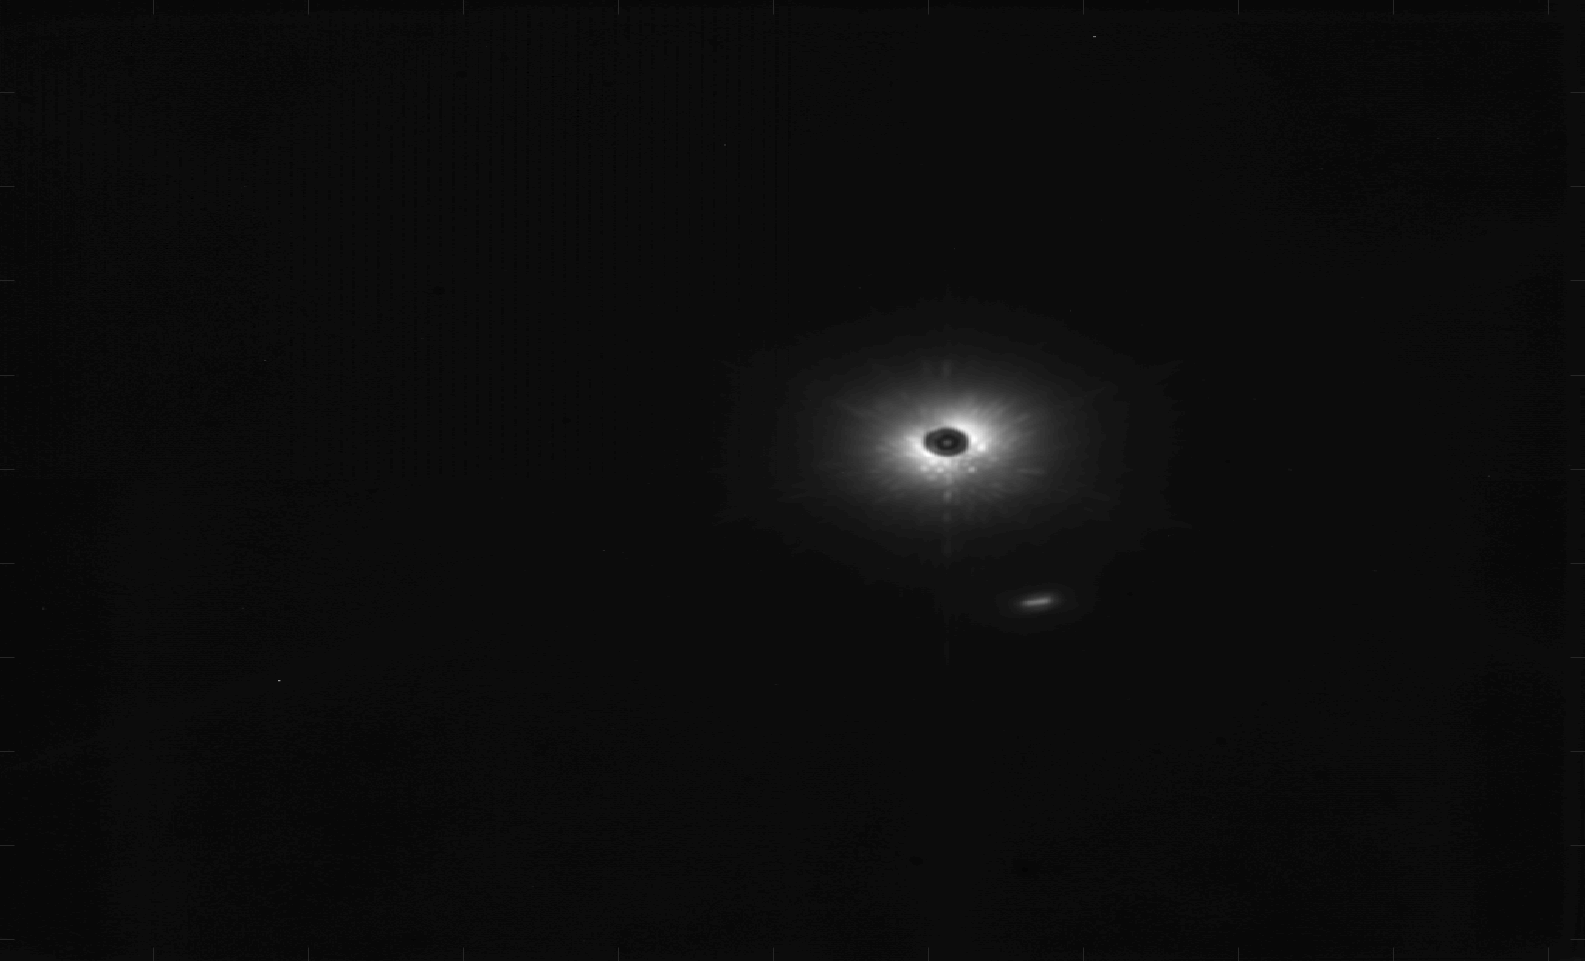
\includegraphics[width=0.45\textwidth]{sum_12.png}
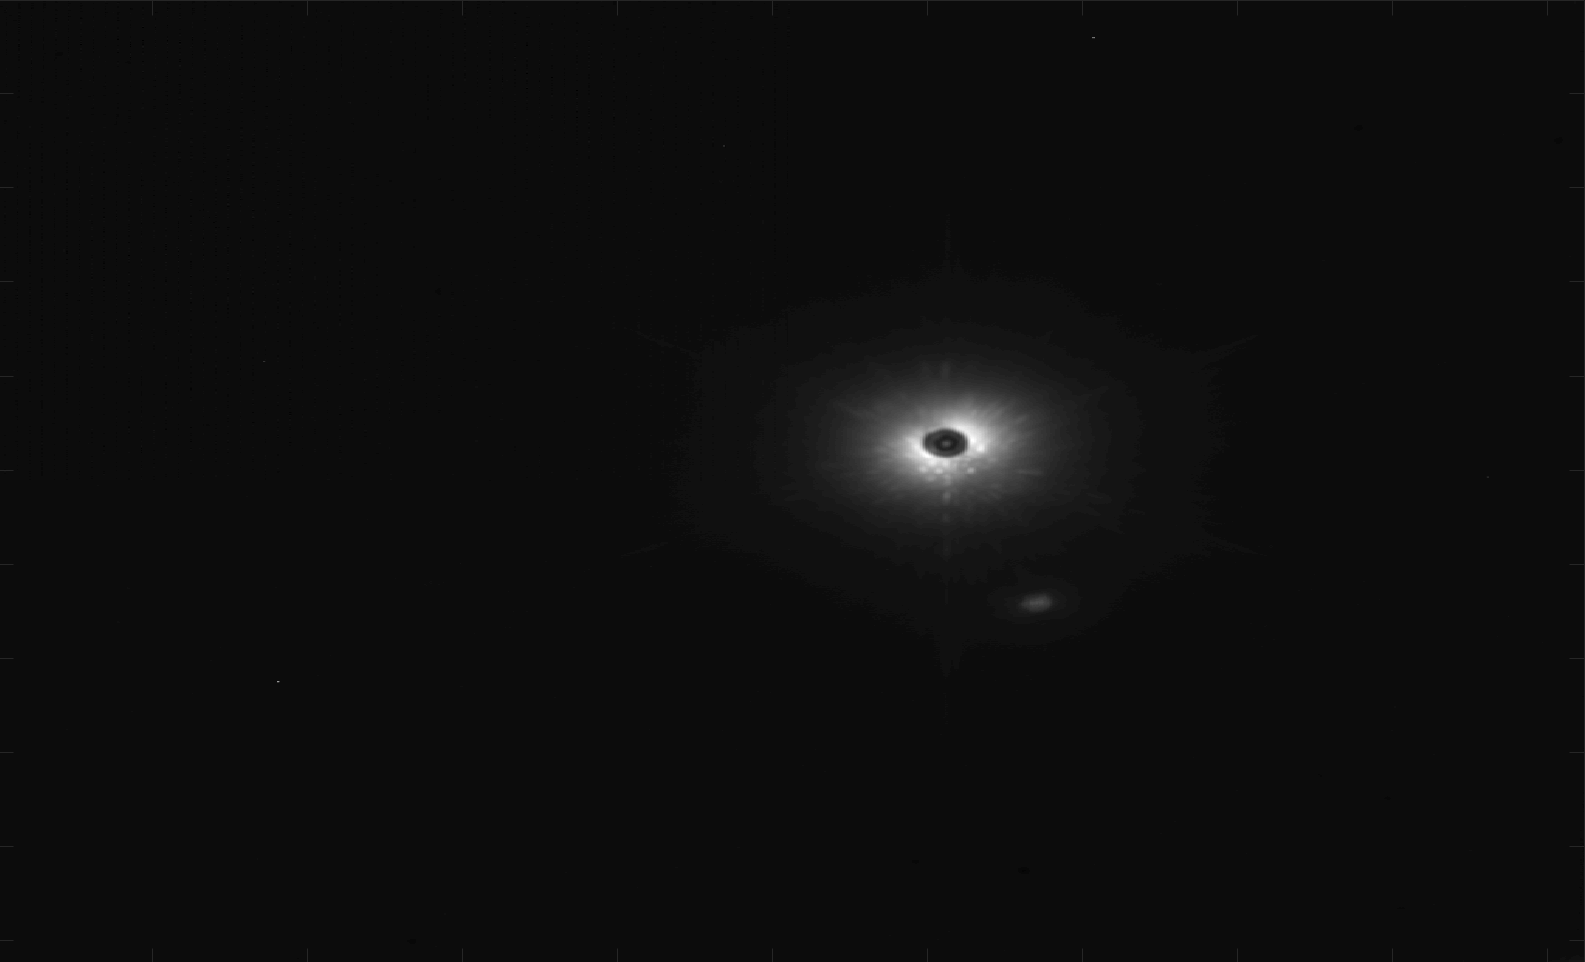
\includegraphics[width=0.45\textwidth]{med_12.png}
\vspace{-1em}
\caption{The sum and median images for ROXs 12.}
\end{figure}
\vspace{-1em}
\begin{figure}[H]
\centering
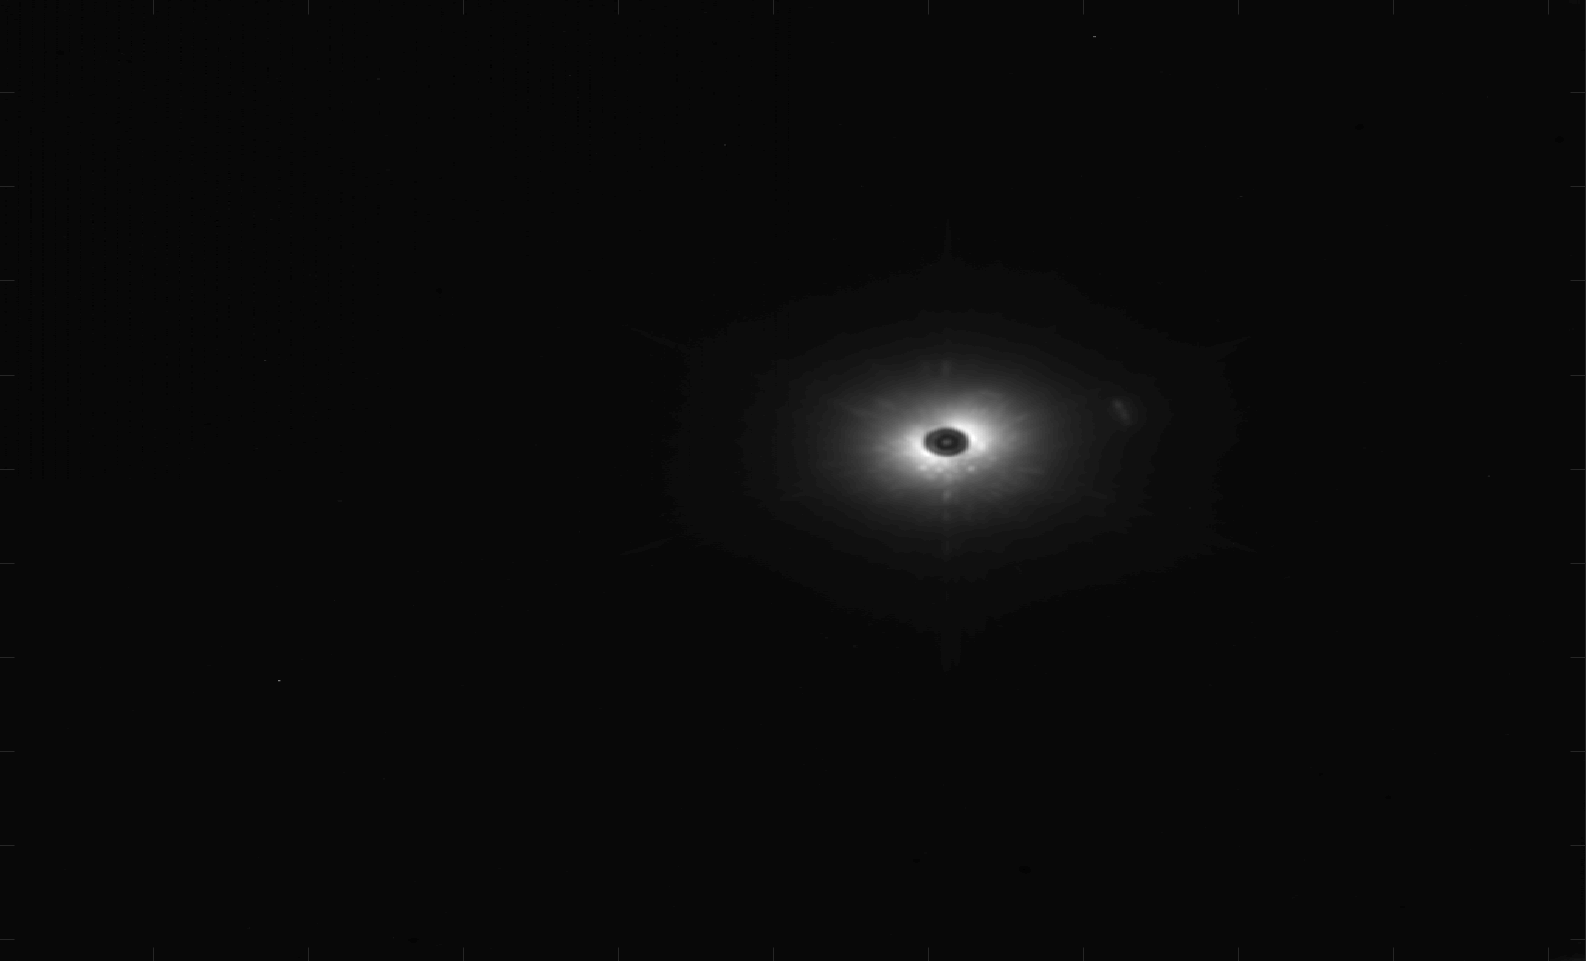
\includegraphics[width=0.45\textwidth]{sum_42b.png}
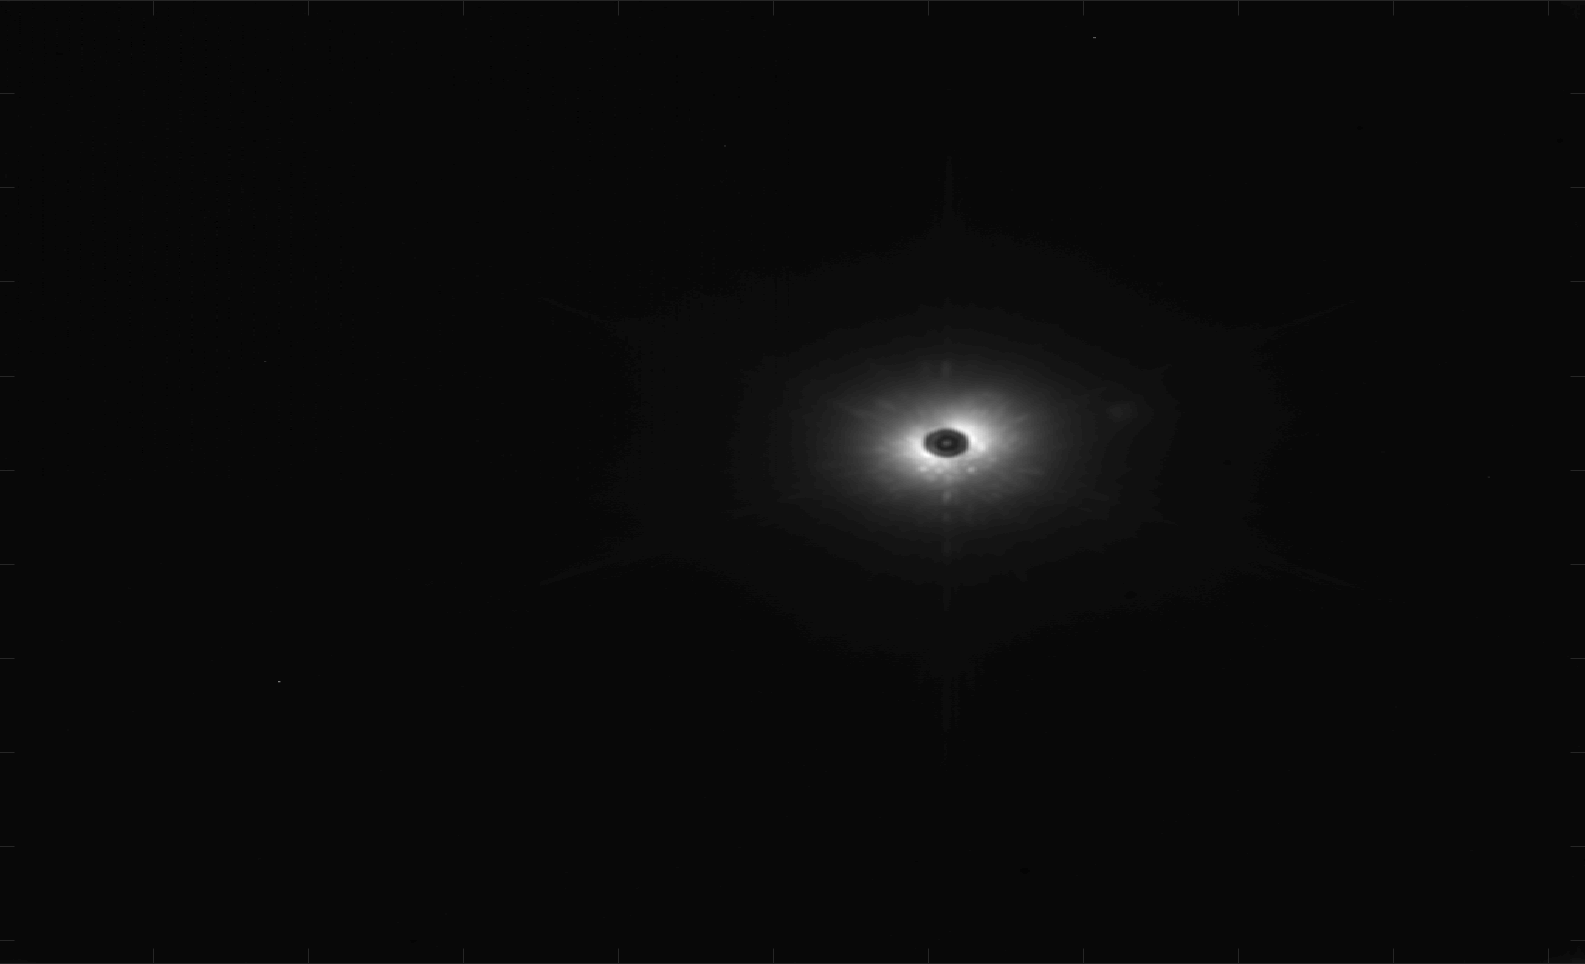
\includegraphics[width=0.45\textwidth]{med_42b.png}
\vspace{-1em}
\caption{The sum and median images for ROXs 42B.}
\end{figure}
\vspace{-1em}
\begin{figure}[H]
\centering
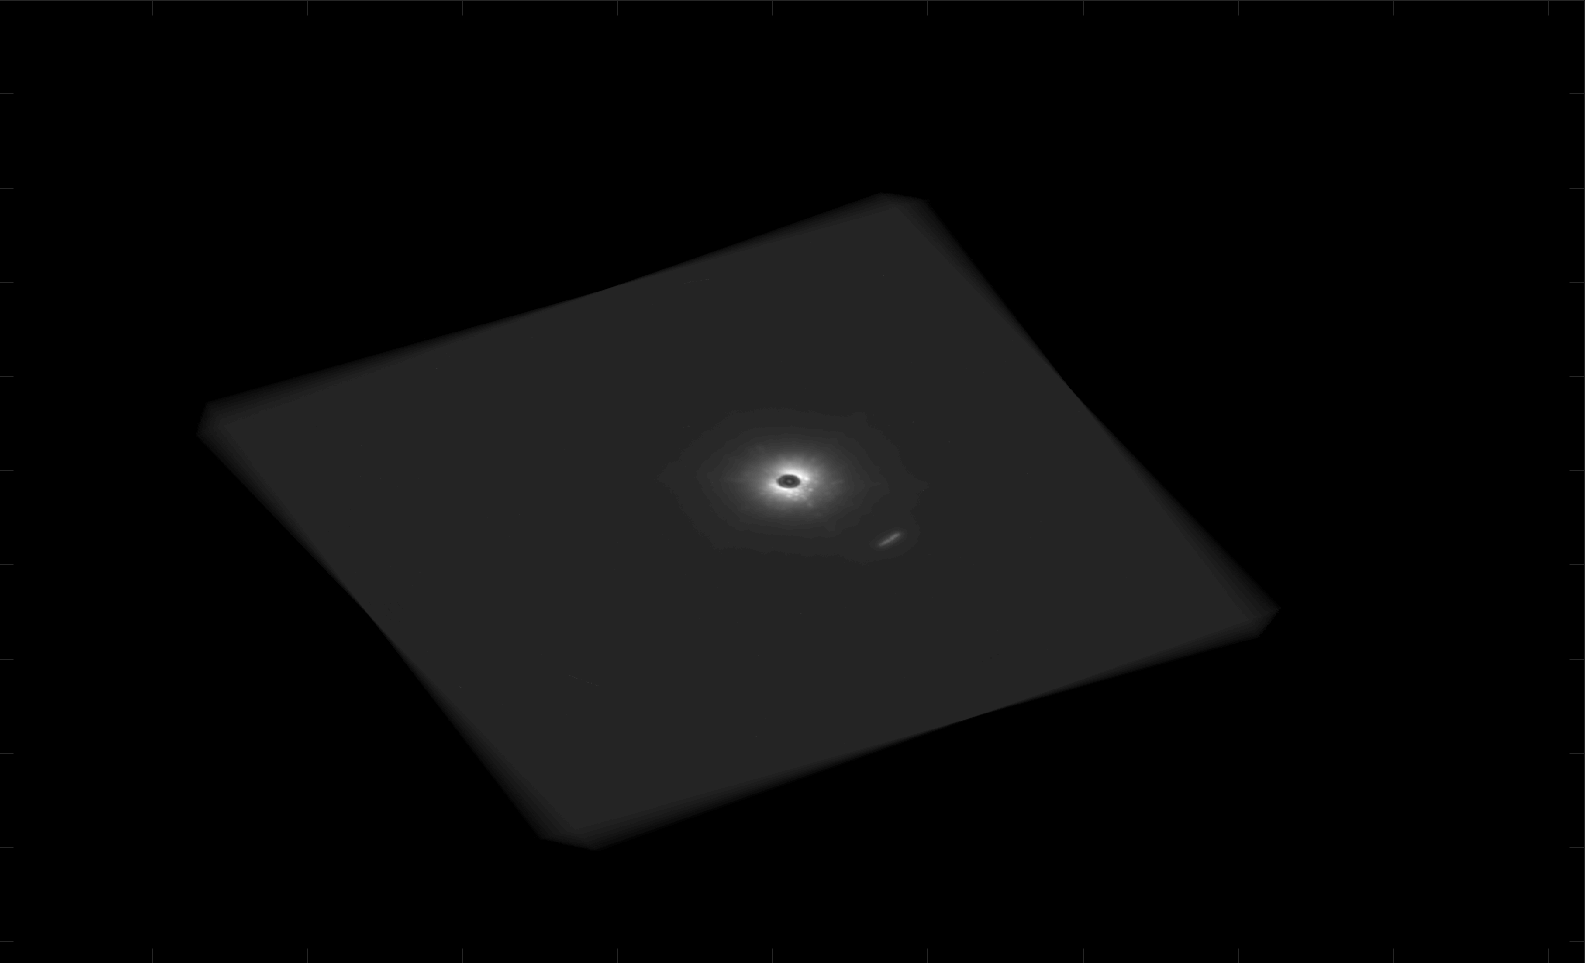
\includegraphics[width=0.45\textwidth]{sum_rot_12.png}
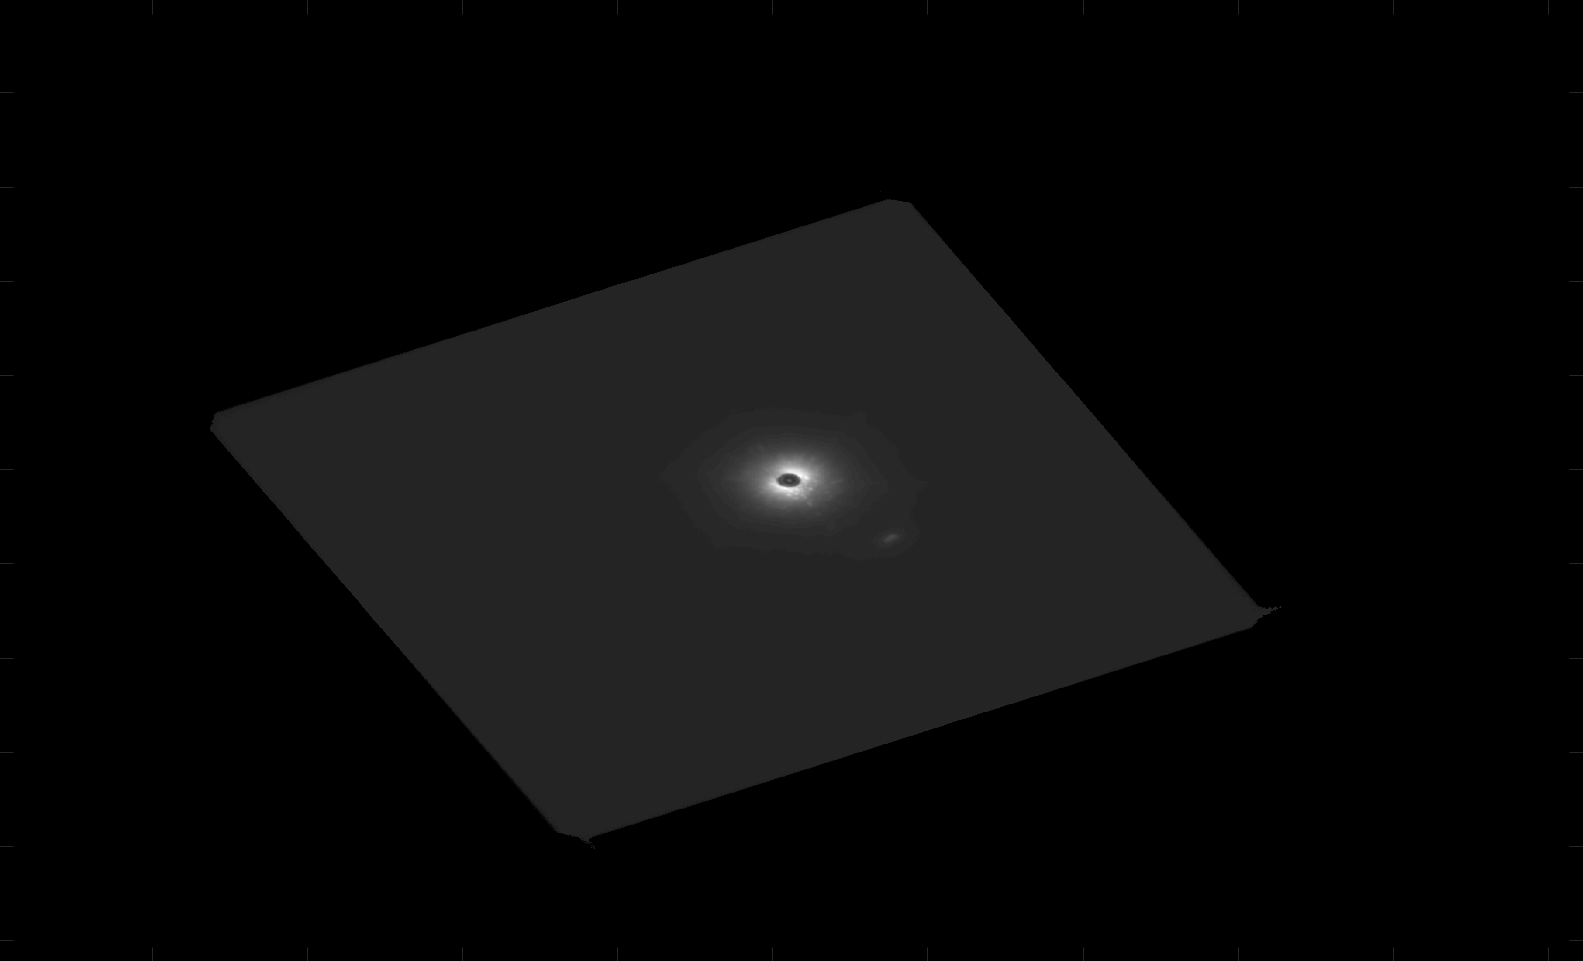
\includegraphics[width=0.45\textwidth]{med_rot_12.png}
\vspace{-1em}
\caption{The sum and median images for ROXs 12, rotated so north is up.}
\end{figure}
\vspace{-1em}
\begin{figure}[H]
\centering
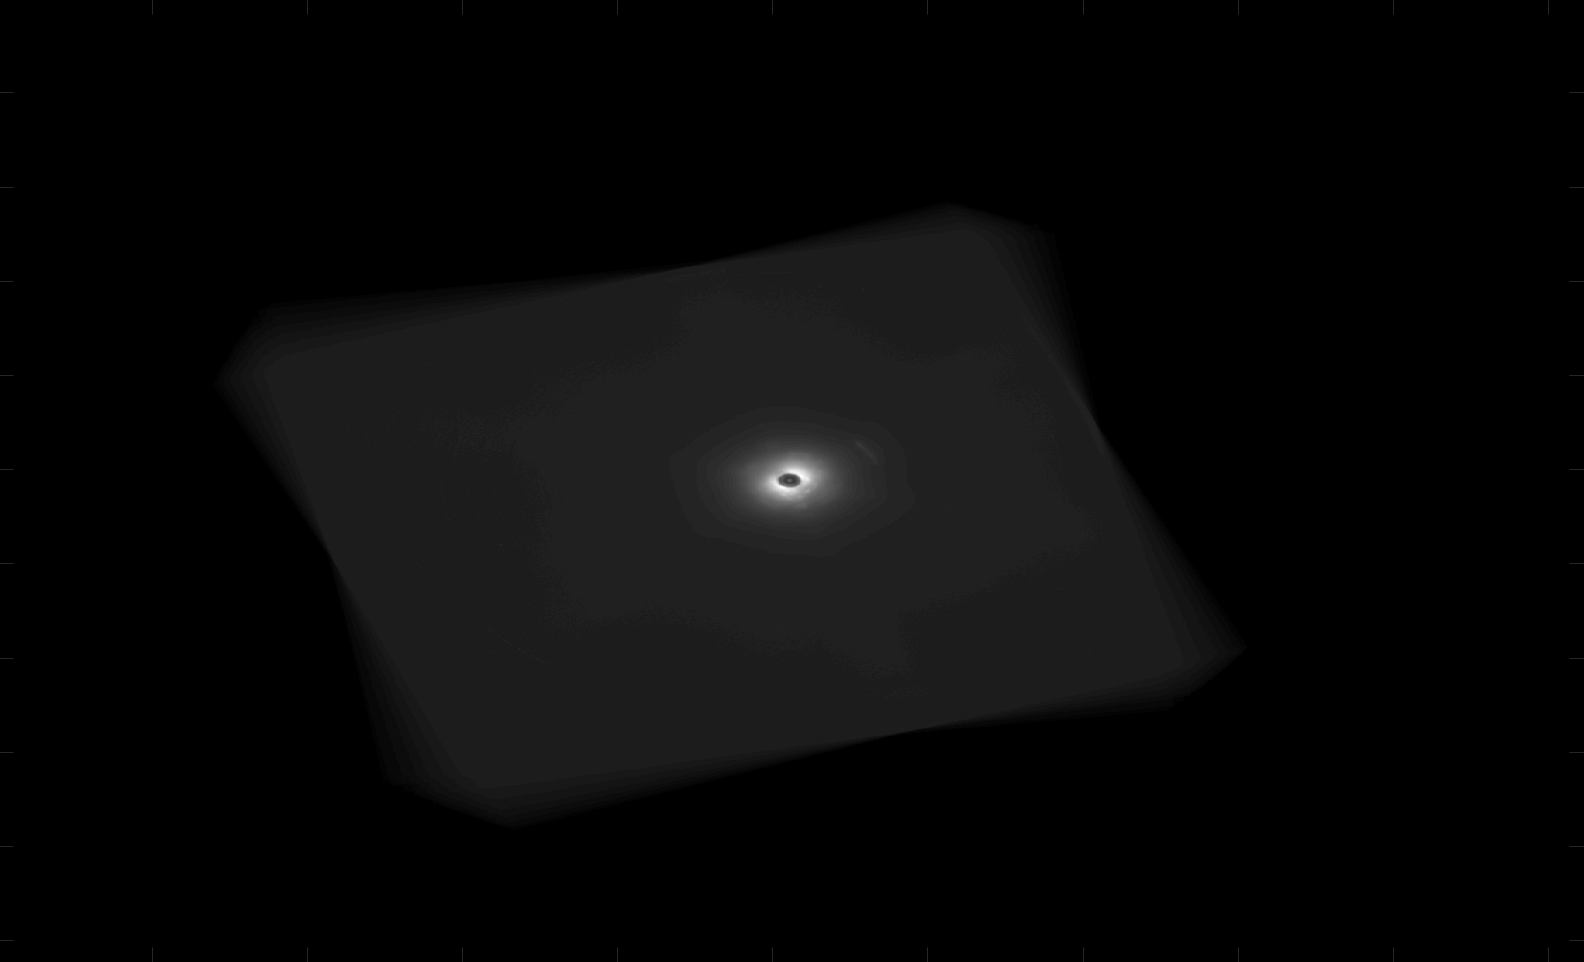
\includegraphics[width=0.45\textwidth]{sum_rot_42b.png}
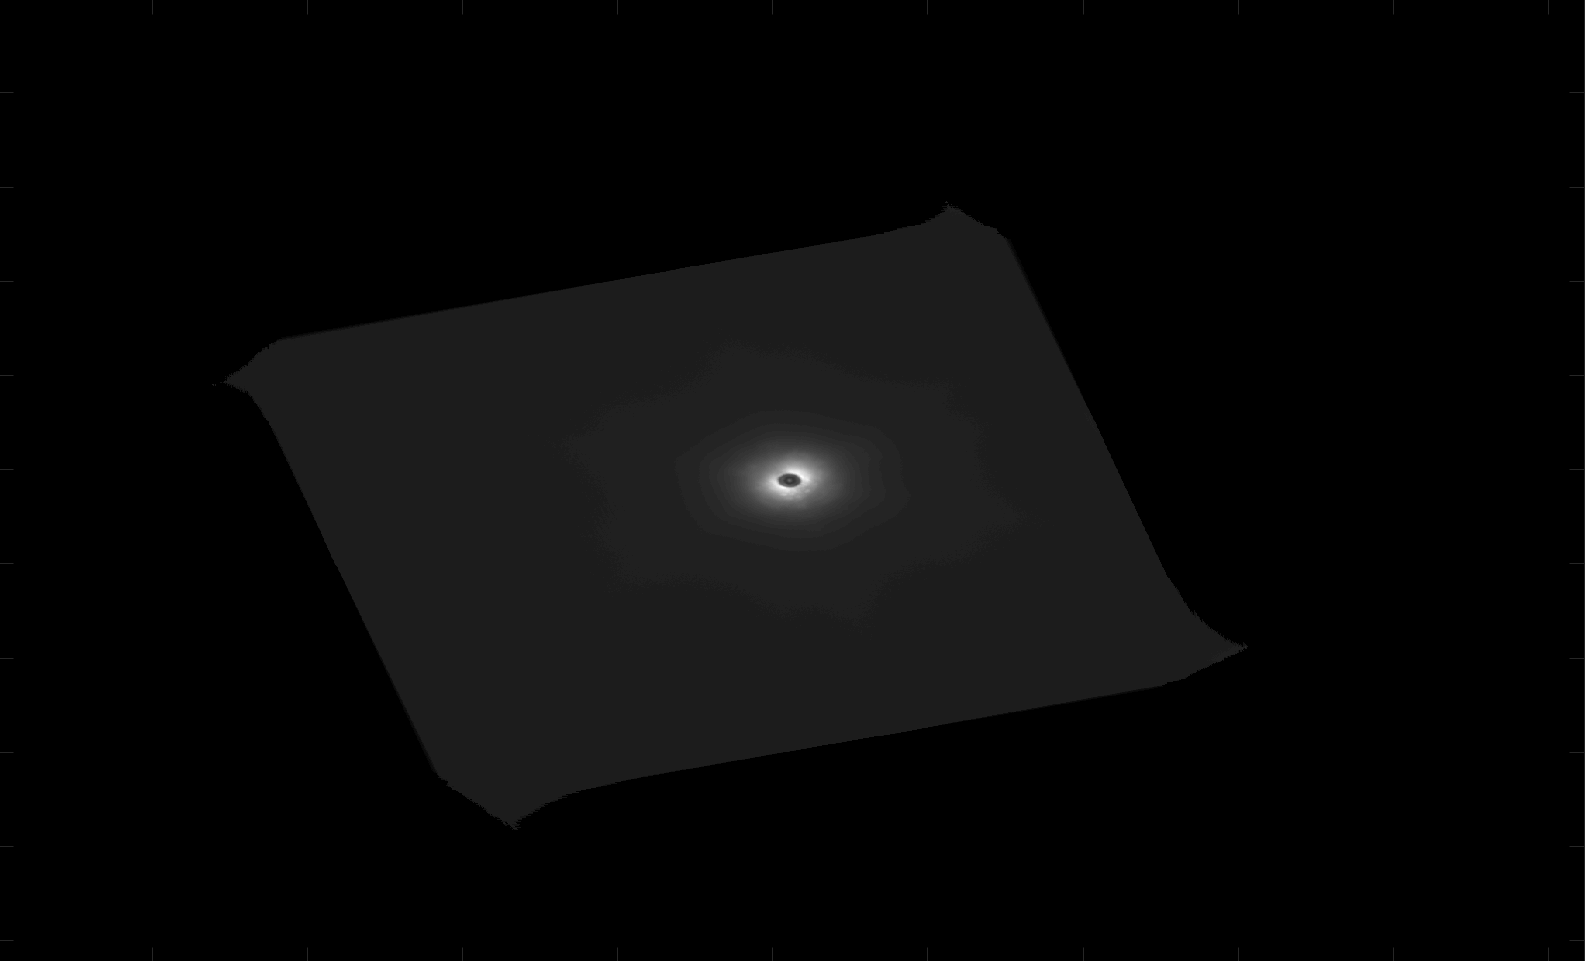
\includegraphics[width=0.45\textwidth]{med_rot_42b.png}
\vspace{-1em}
\caption{The sum and median images for ROXs 42B, rotated so north is up.}
\end{figure}
\vspace{-1em}
\begin{figure}[H]
\centering
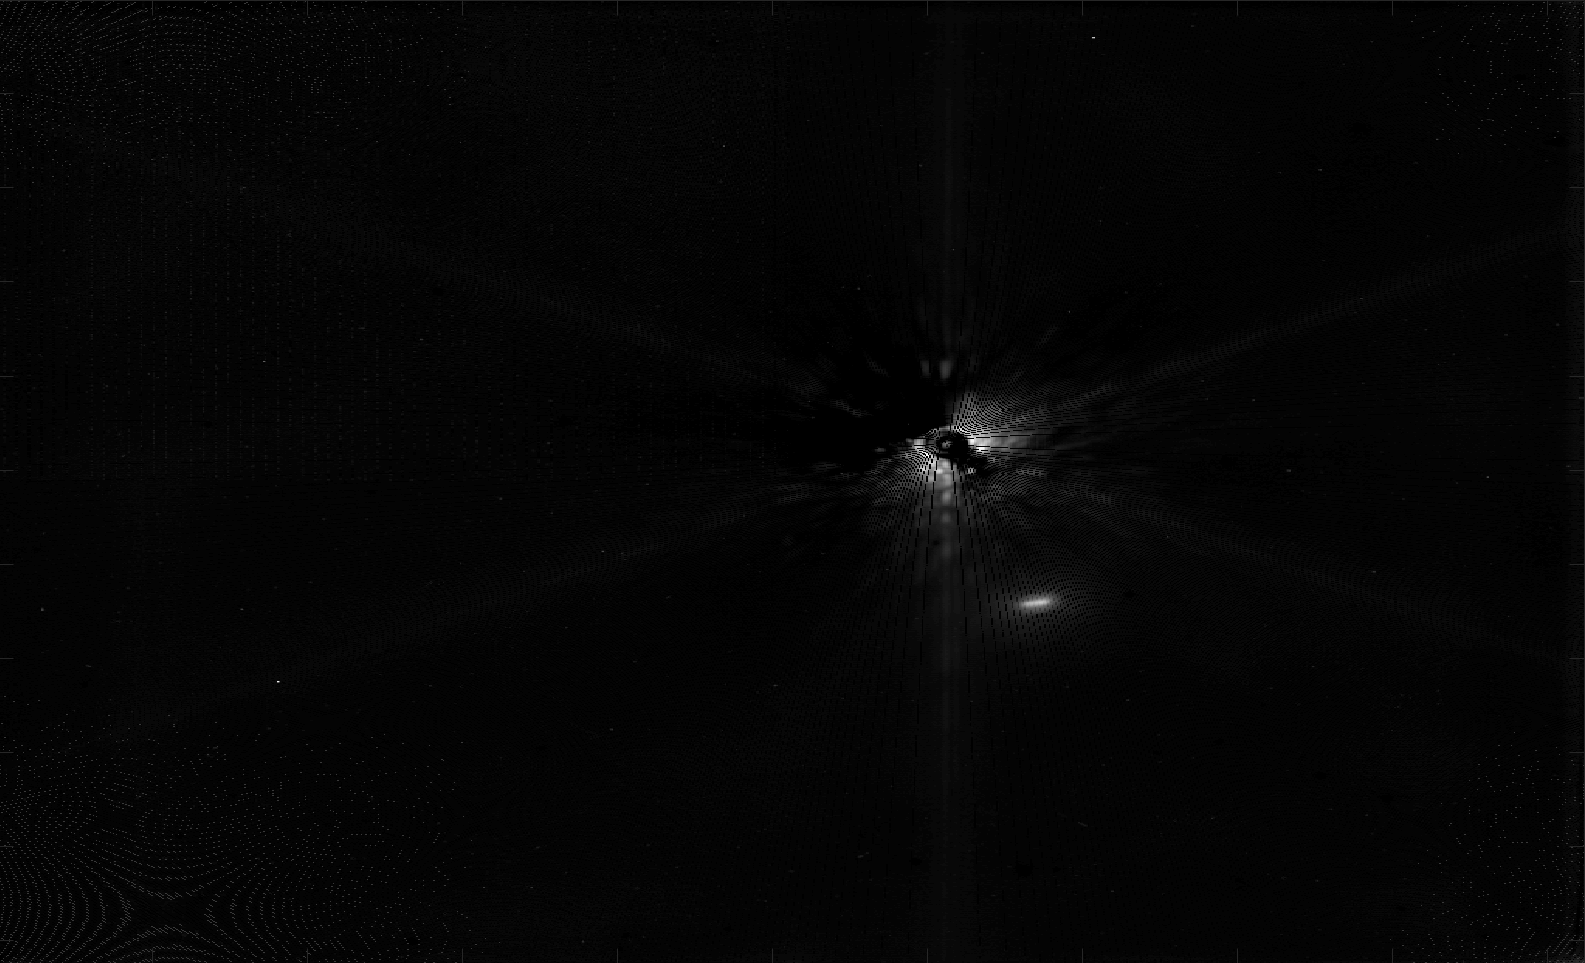
\includegraphics[width=0.45\textwidth]{sum_sub_12.png}
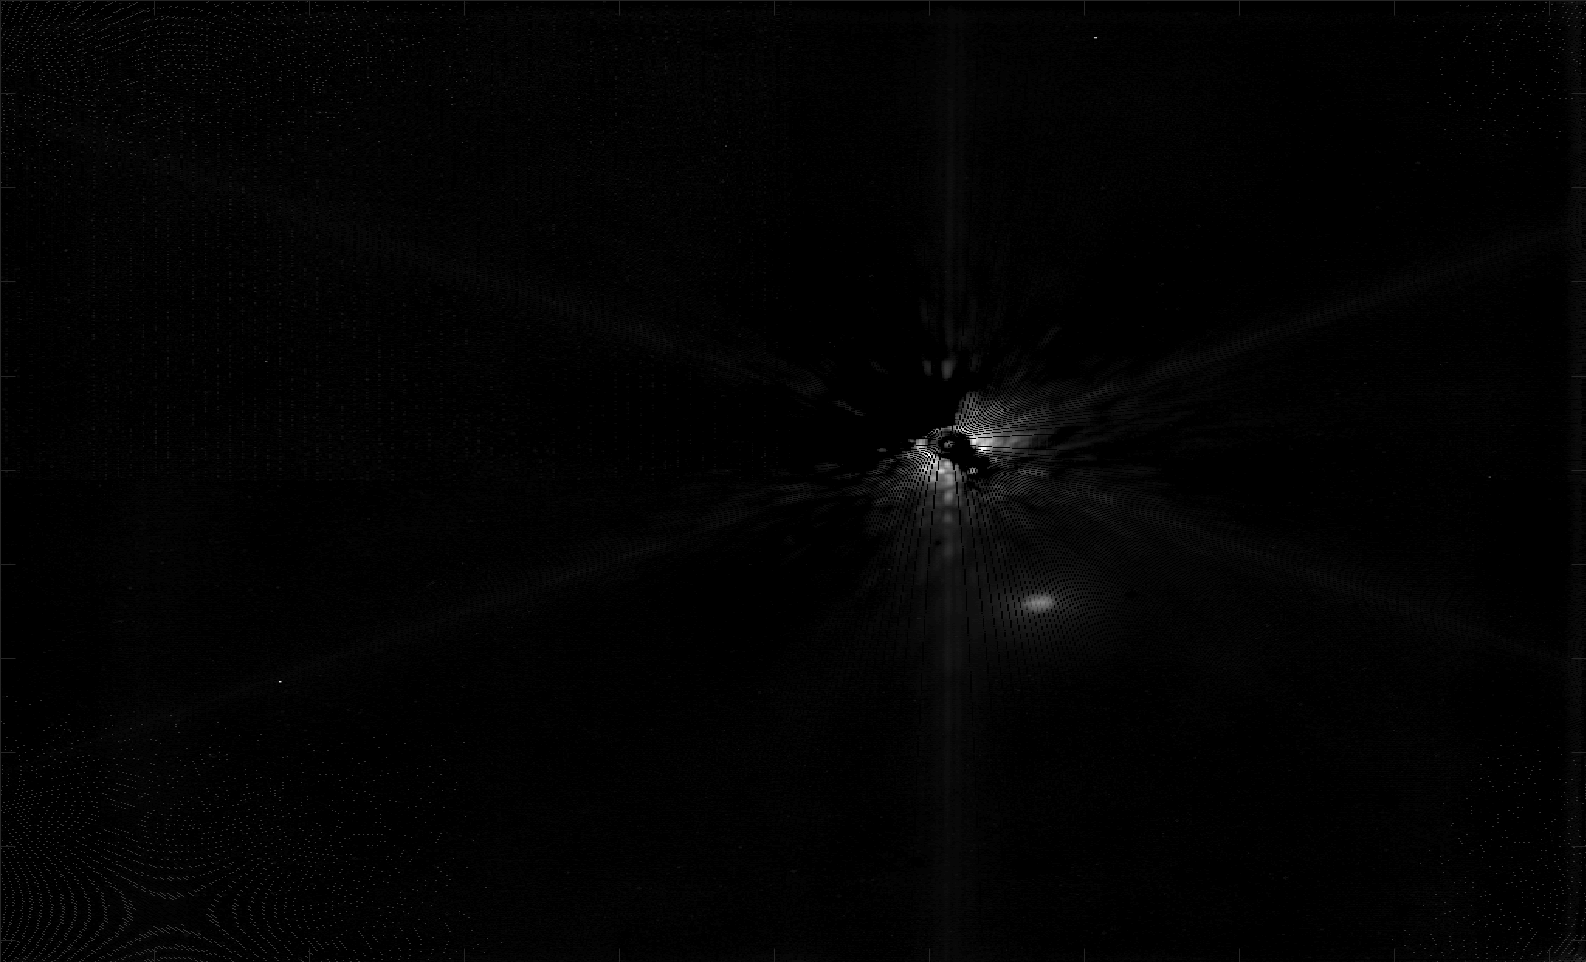
\includegraphics[width=0.45\textwidth]{med_sub_12.png}
\vspace{-1em}
\caption{The sum and median images for ROXs 12, subtracting the brightness profile.}
\end{figure}
\vspace{-1em}
\begin{figure}[H]
\centering
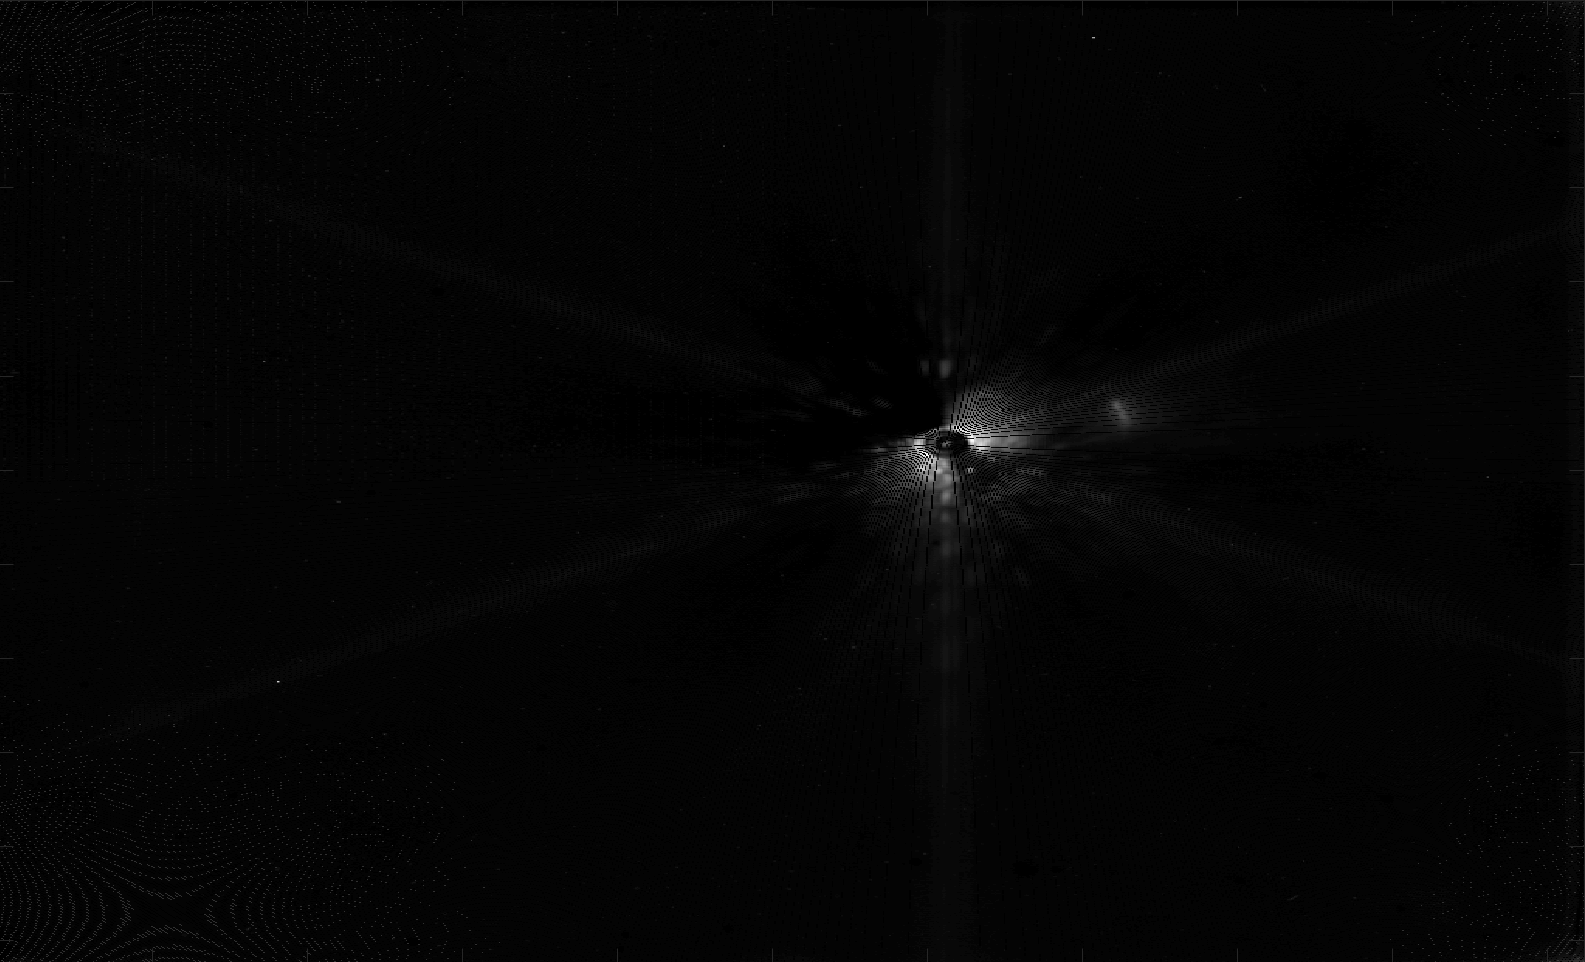
\includegraphics[width=0.45\textwidth]{sum_sub_42b.png}
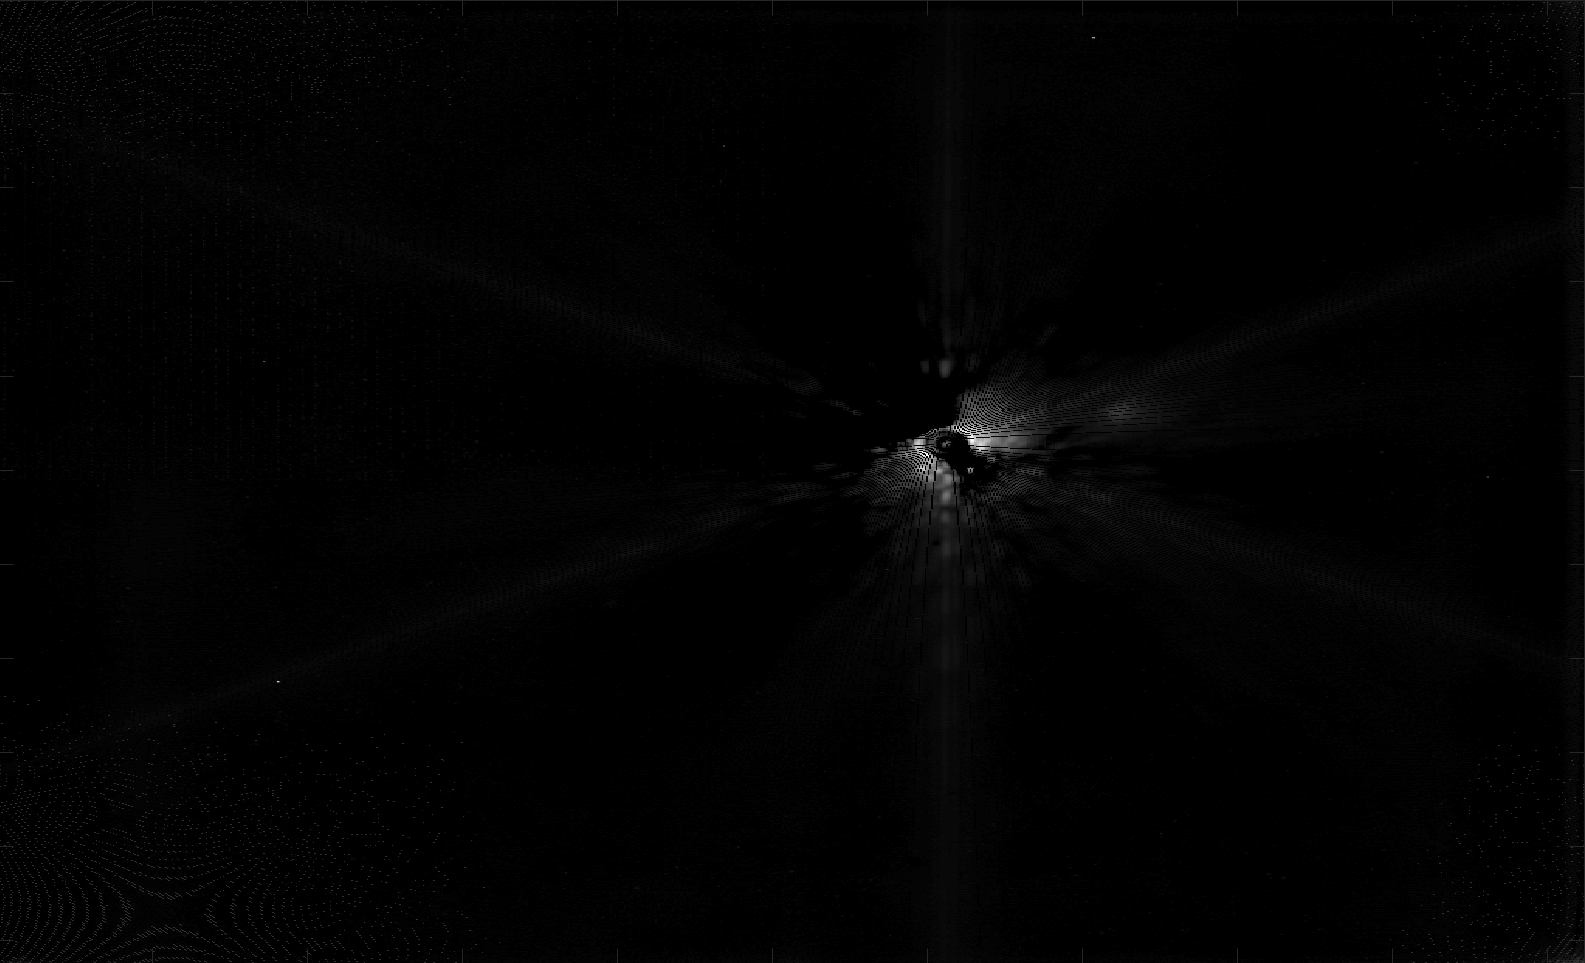
\includegraphics[width=0.45\textwidth]{med_sub_42b.png}
\vspace{-1em}
\caption{The sum and median images for ROXs 42B, subtracting the brightness profile.}
\end{figure}
\vspace{-1em}
\begin{figure}[H]
\centering
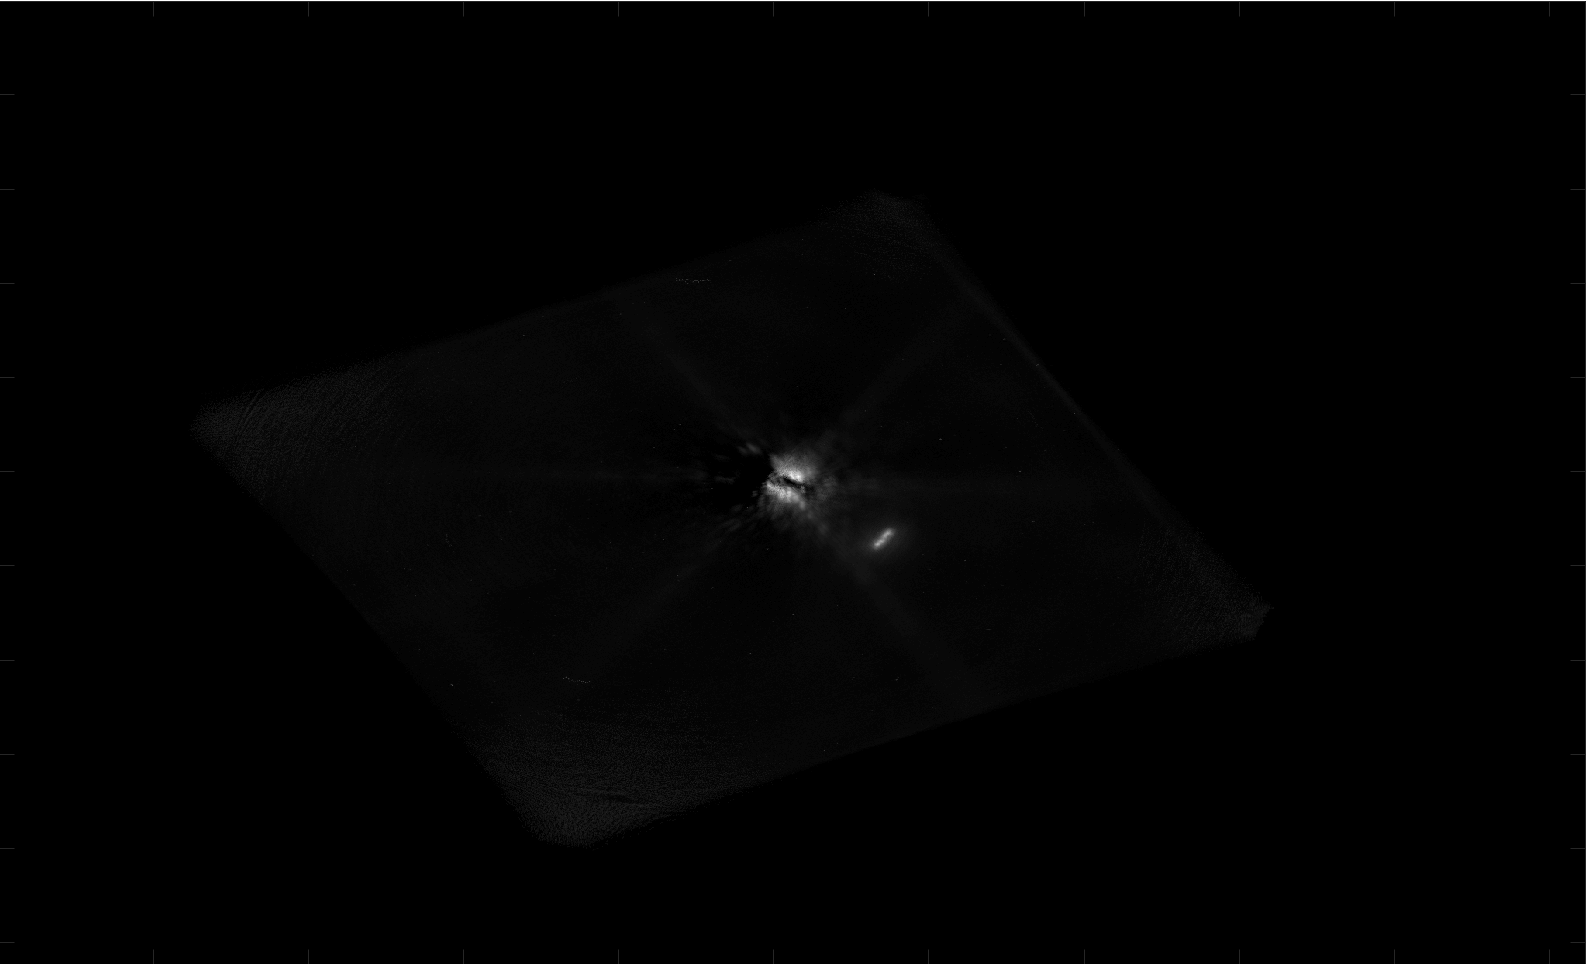
\includegraphics[width=0.45\textwidth]{sum_rot_sub_12.png}
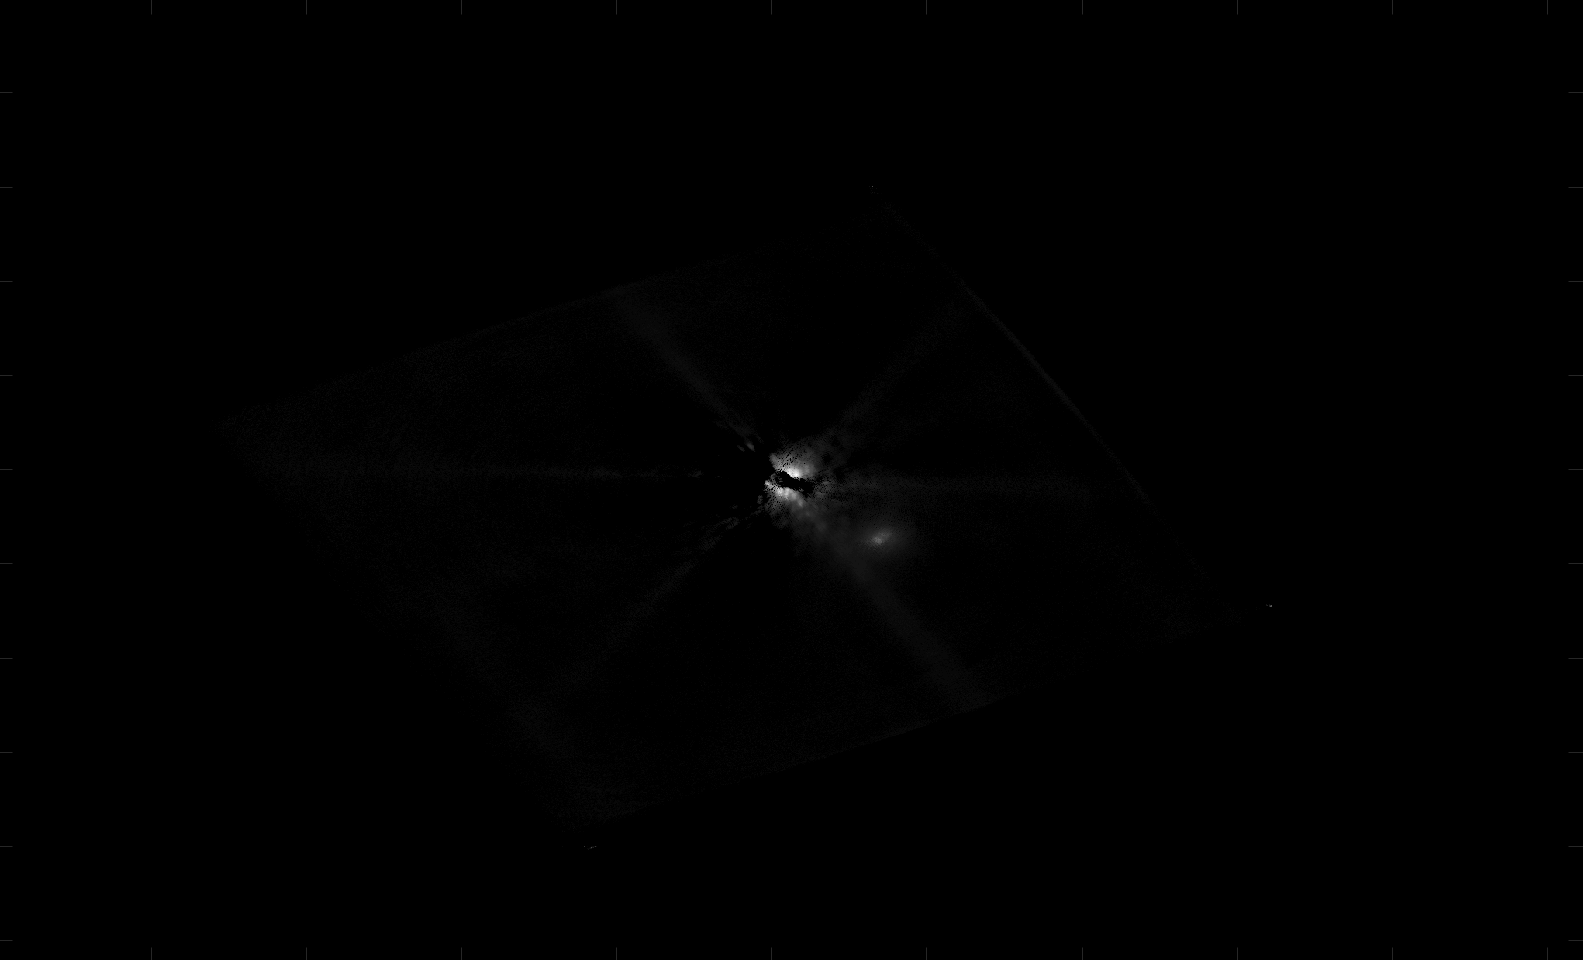
\includegraphics[width=0.45\textwidth]{med_rot_sub_12.png}
\vspace{-1em}
\caption{The sum and median images for ROXs 12, rotated so north is up and subtracting the brightness profile.}
\end{figure}
\vspace{-1em}
\begin{figure}[H]
\centering
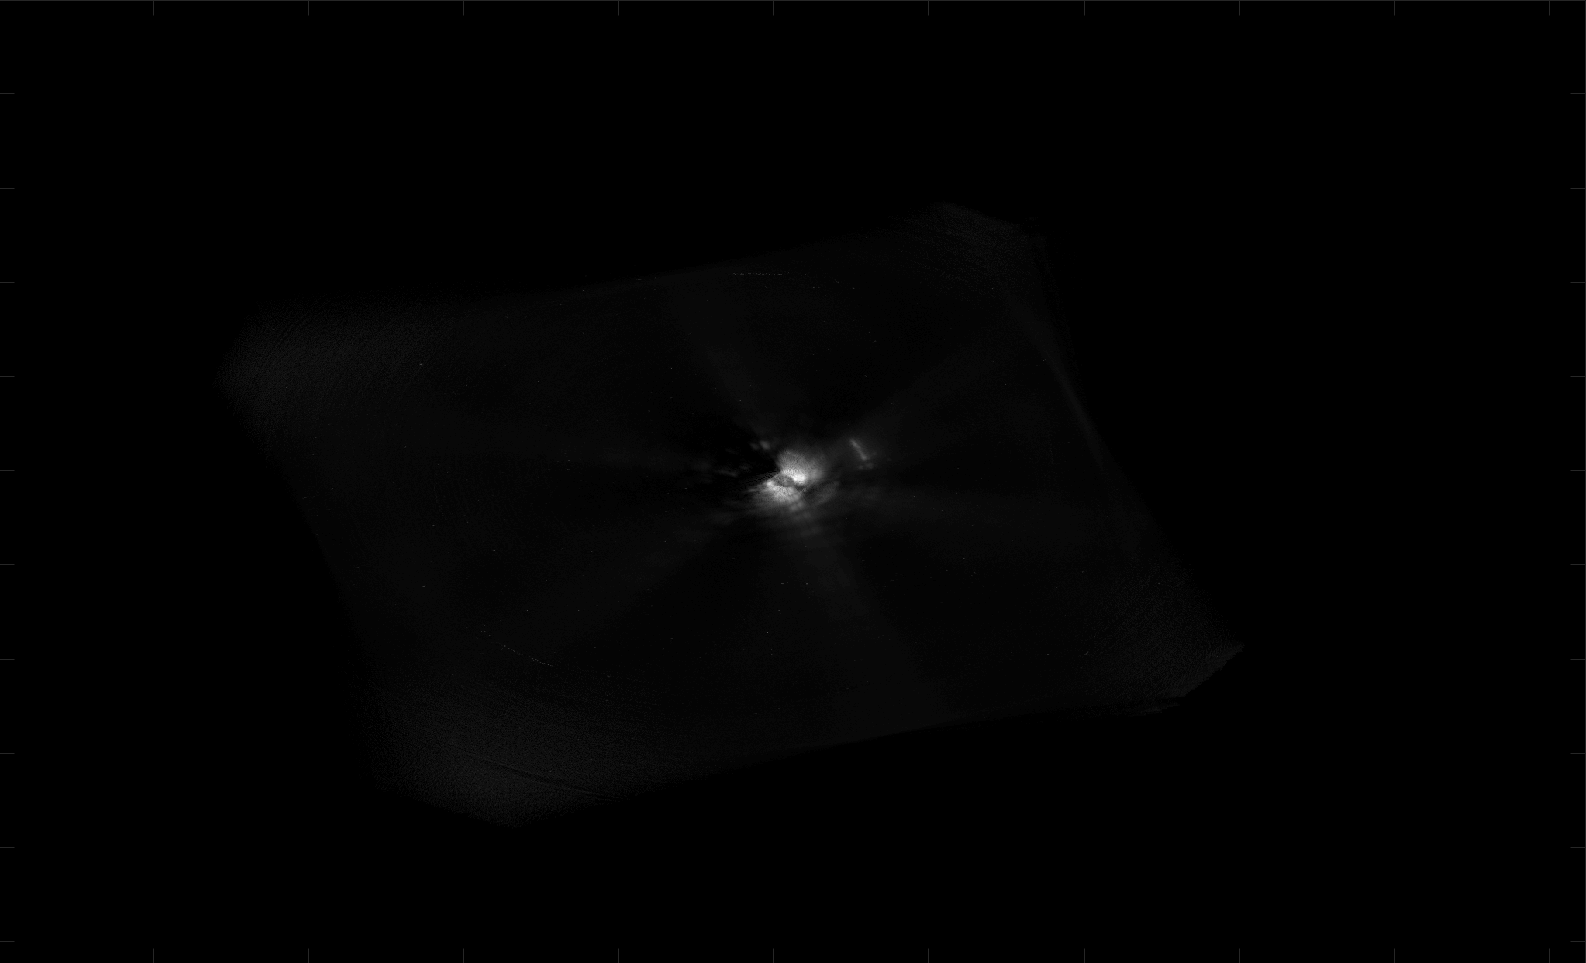
\includegraphics[width=0.45\textwidth]{sum_rot_sub_42b.png}
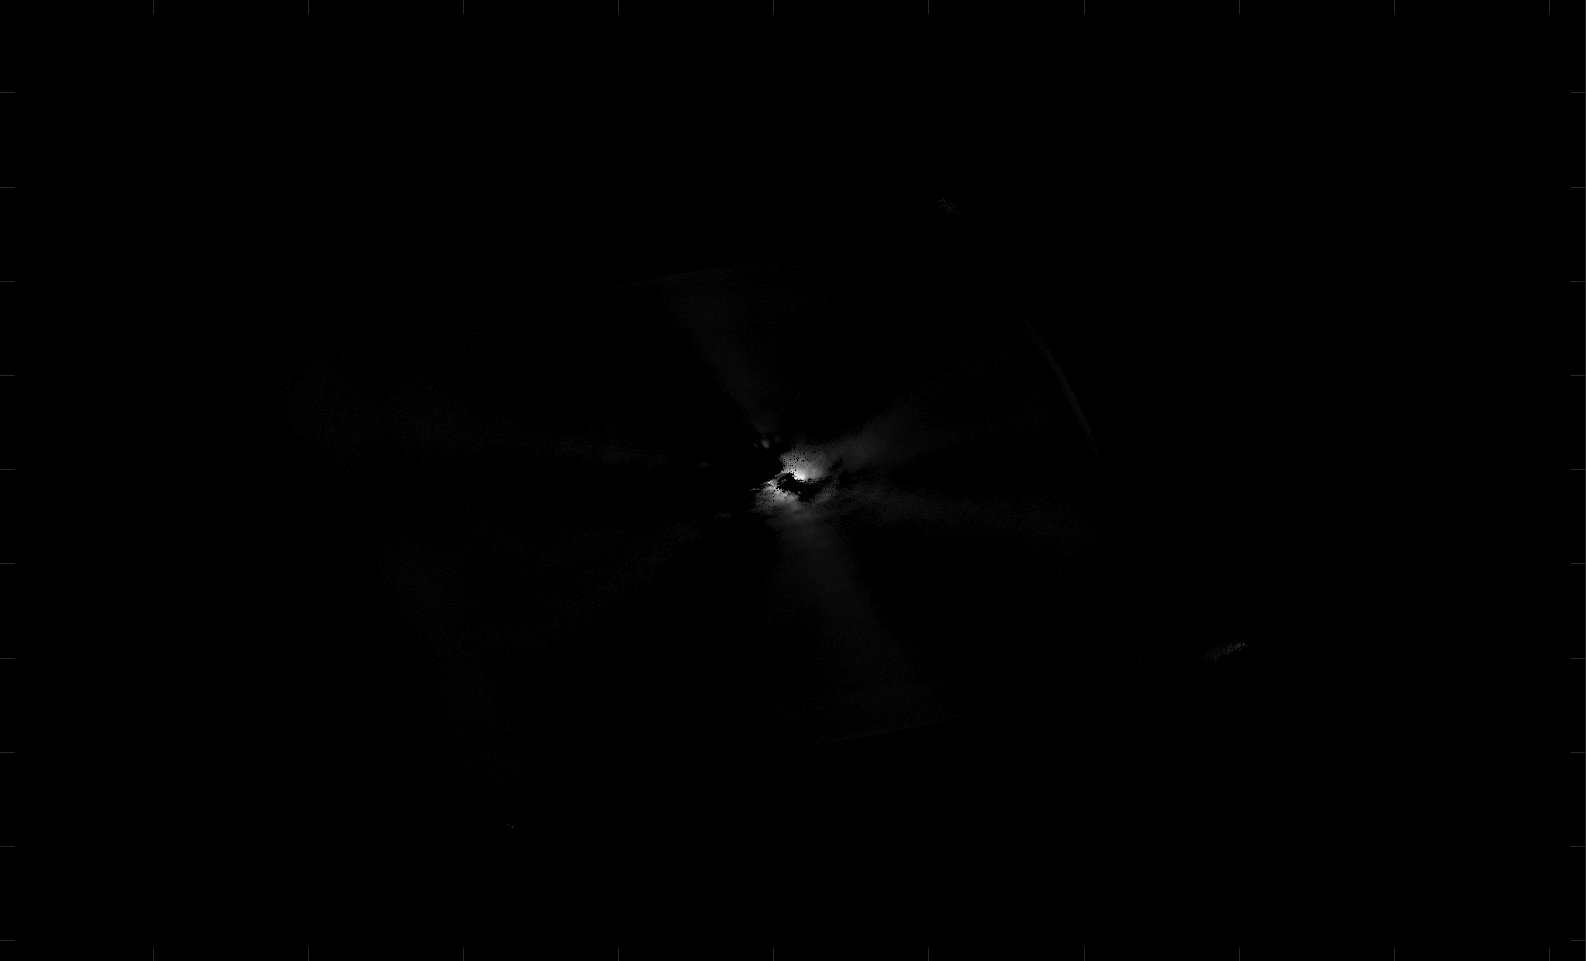
\includegraphics[width=0.45\textwidth]{med_rot_sub_42b.png}
\vspace{-1em}
\caption{The sum and median images for ROXs 42B, rotated so north is up and subtracting the brightness profile.}
\end{figure}
\vspace{-1em}
\begin{figure}[H]
\centering
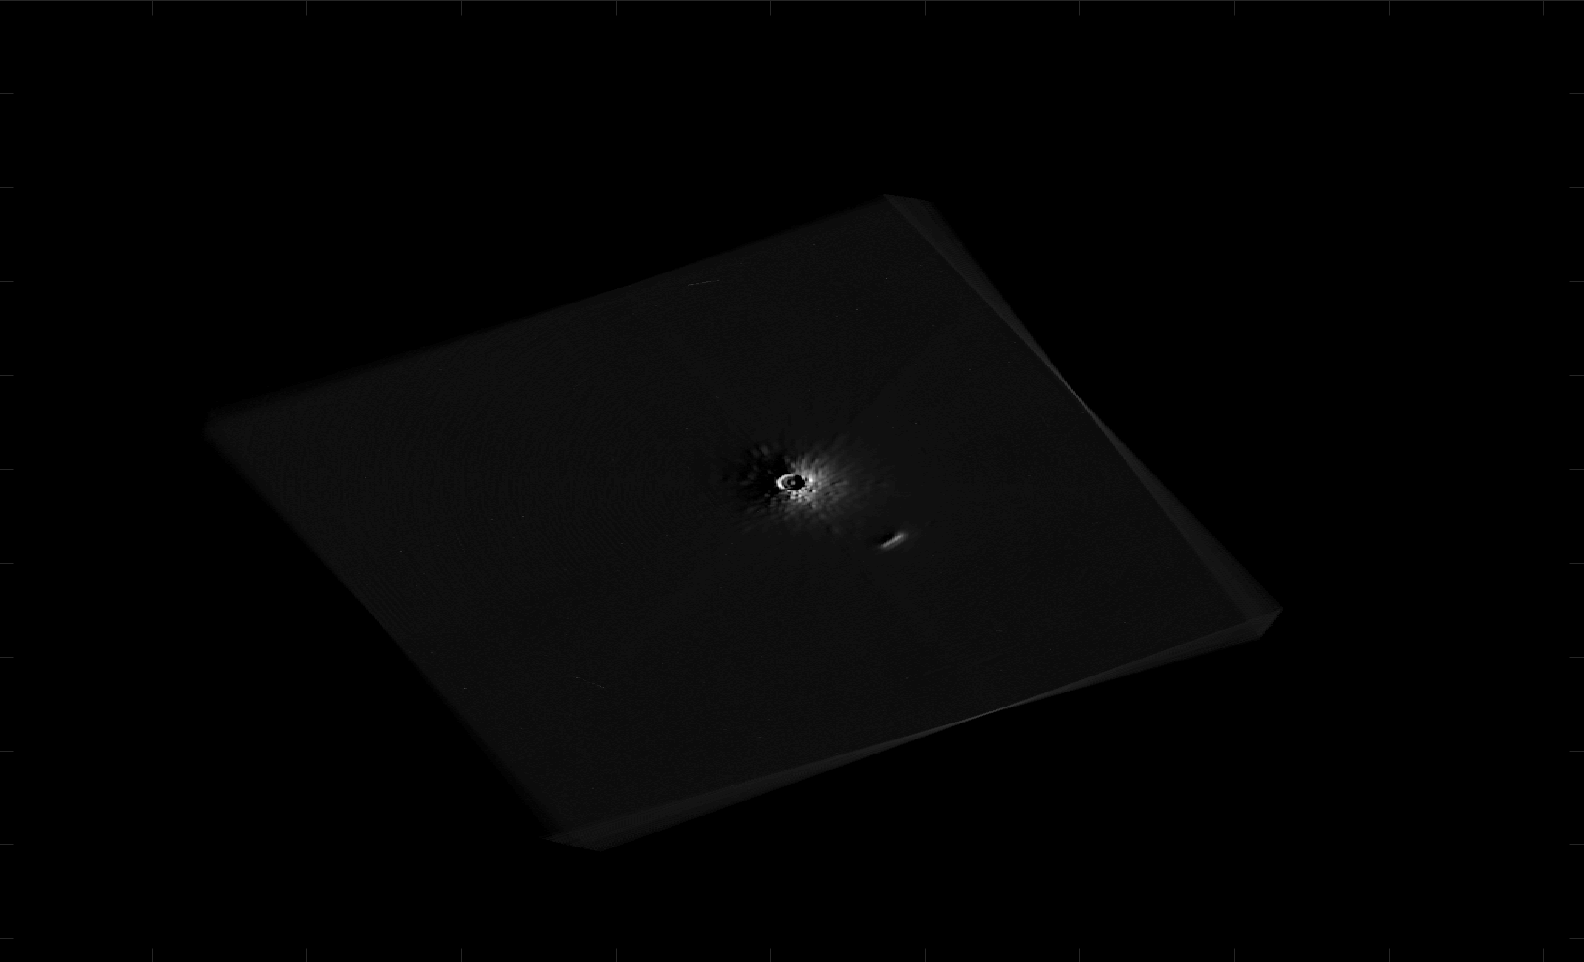
\includegraphics[width=0.45\textwidth]{sum_rot_adi_12.png}
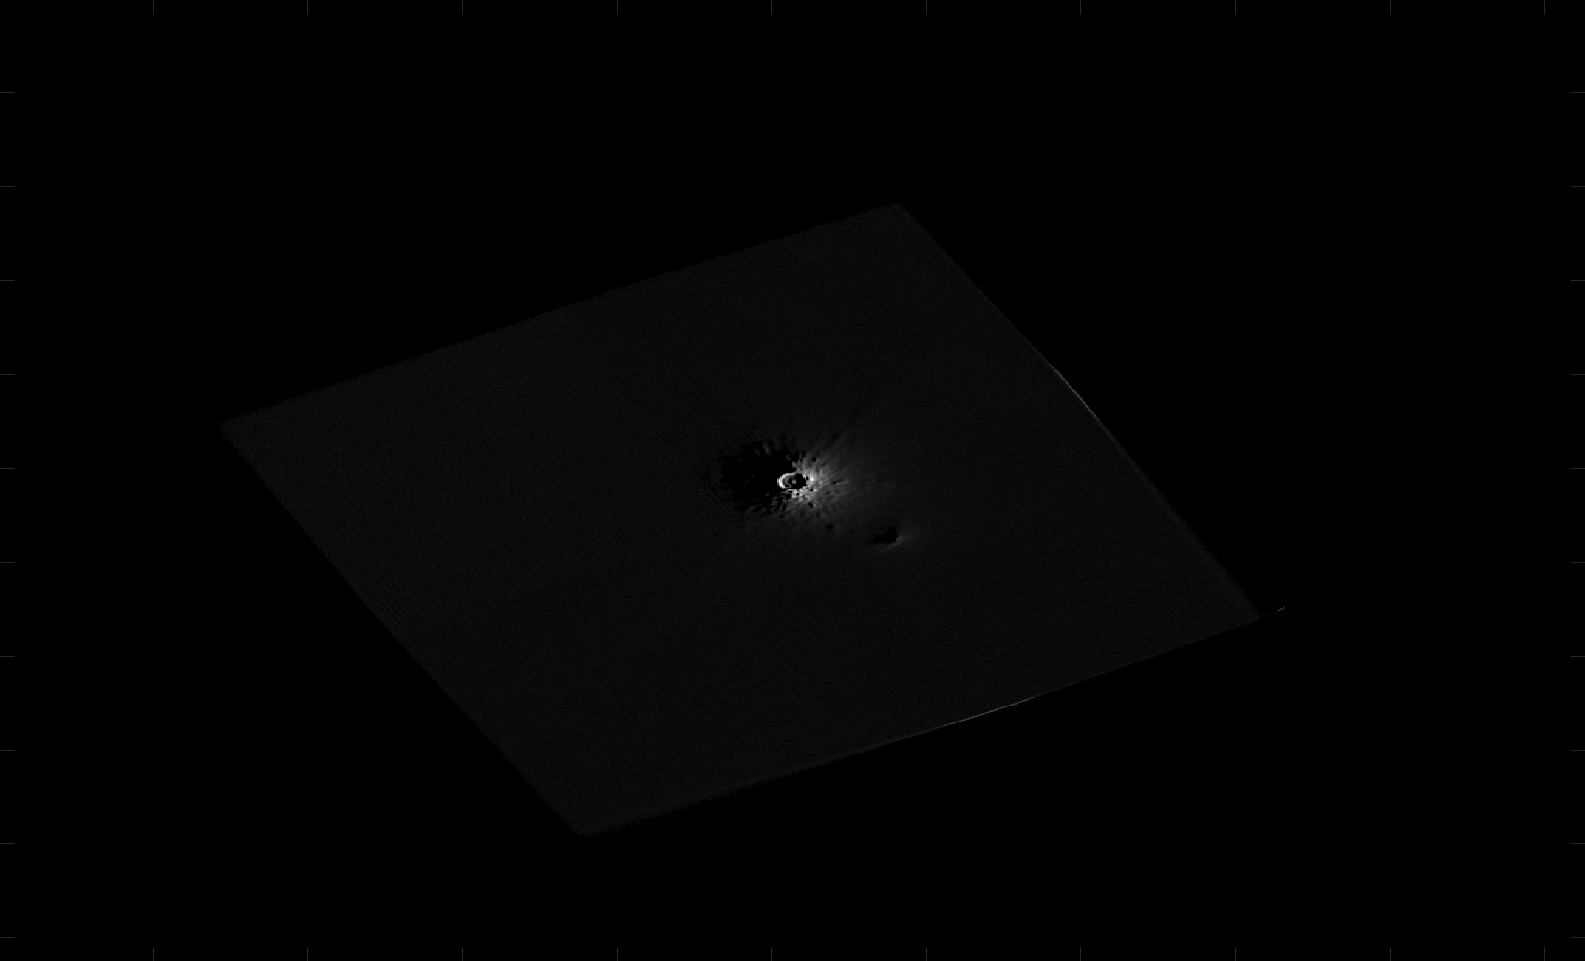
\includegraphics[width=0.45\textwidth]{med_rot_adi_12.png}
\vspace{-1em}
\caption{The sum and median images for ROXs 12, rotated so north is up and subtracting the median PSF.}
\end{figure}
\vspace{-1em}
\begin{figure}[H]
\centering
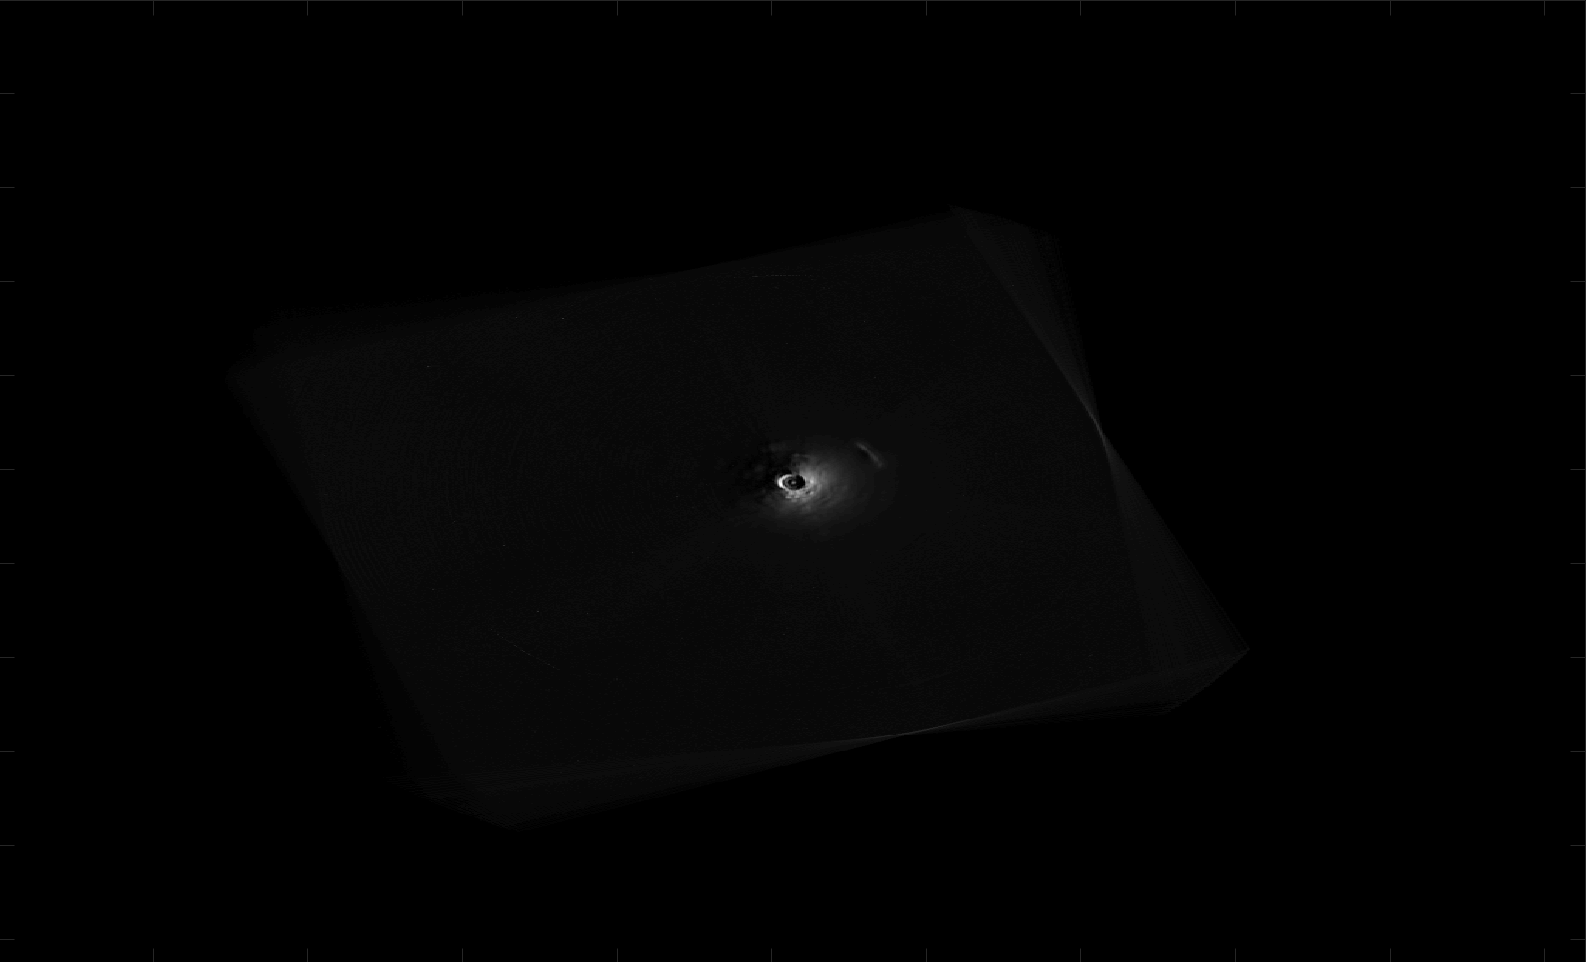
\includegraphics[width=0.45\textwidth]{sum_rot_adi_42b.png}
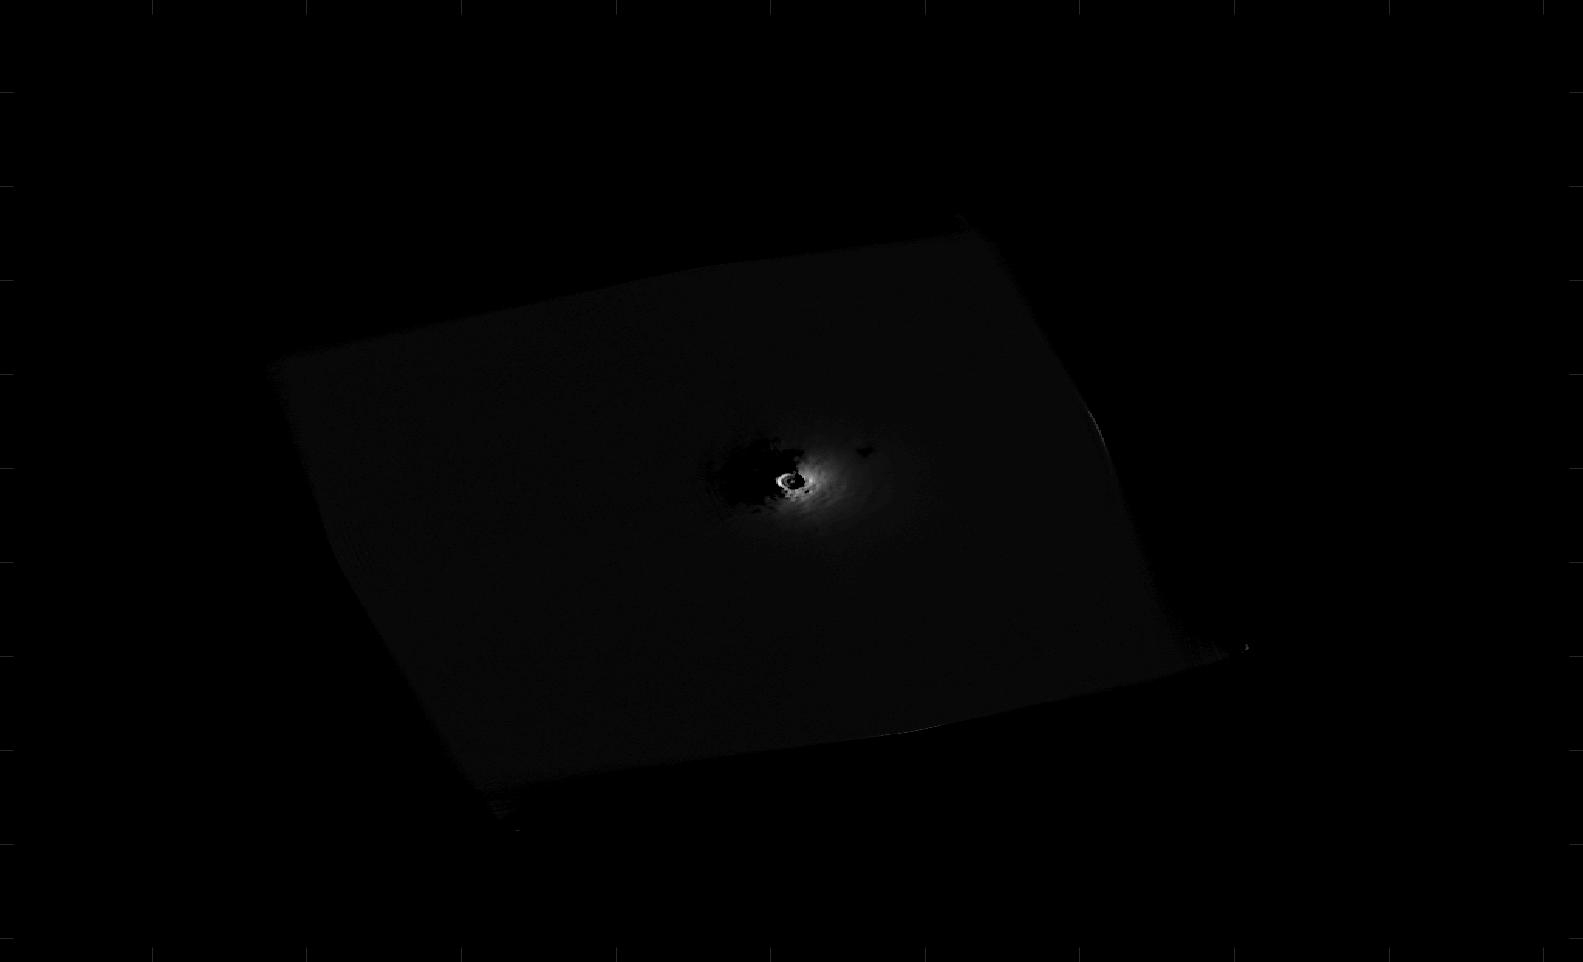
\includegraphics[width=0.45\textwidth]{med_rot_adi_42b.png}
\vspace{-1em}
\caption{The sum and median images for ROXs 42B, rotated so north is up and subtracting the median PSF.}
\end{figure}
\vspace{-1em}
\begin{figure}[H]
\centering
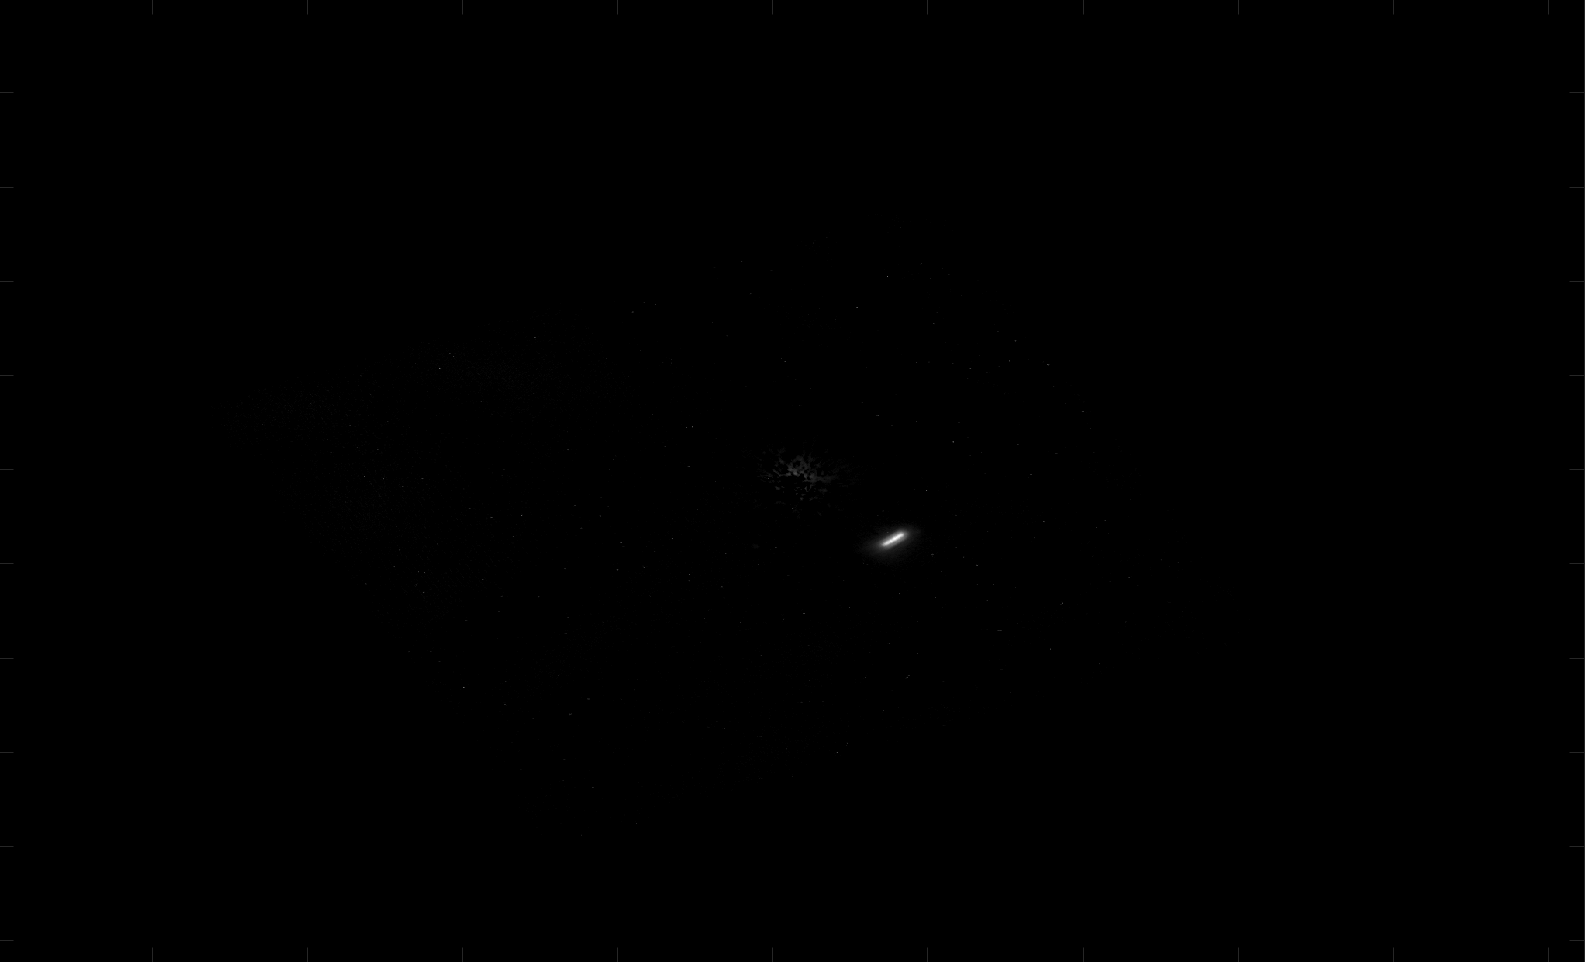
\includegraphics[width=0.45\textwidth]{sum_rot_psf_12.png}
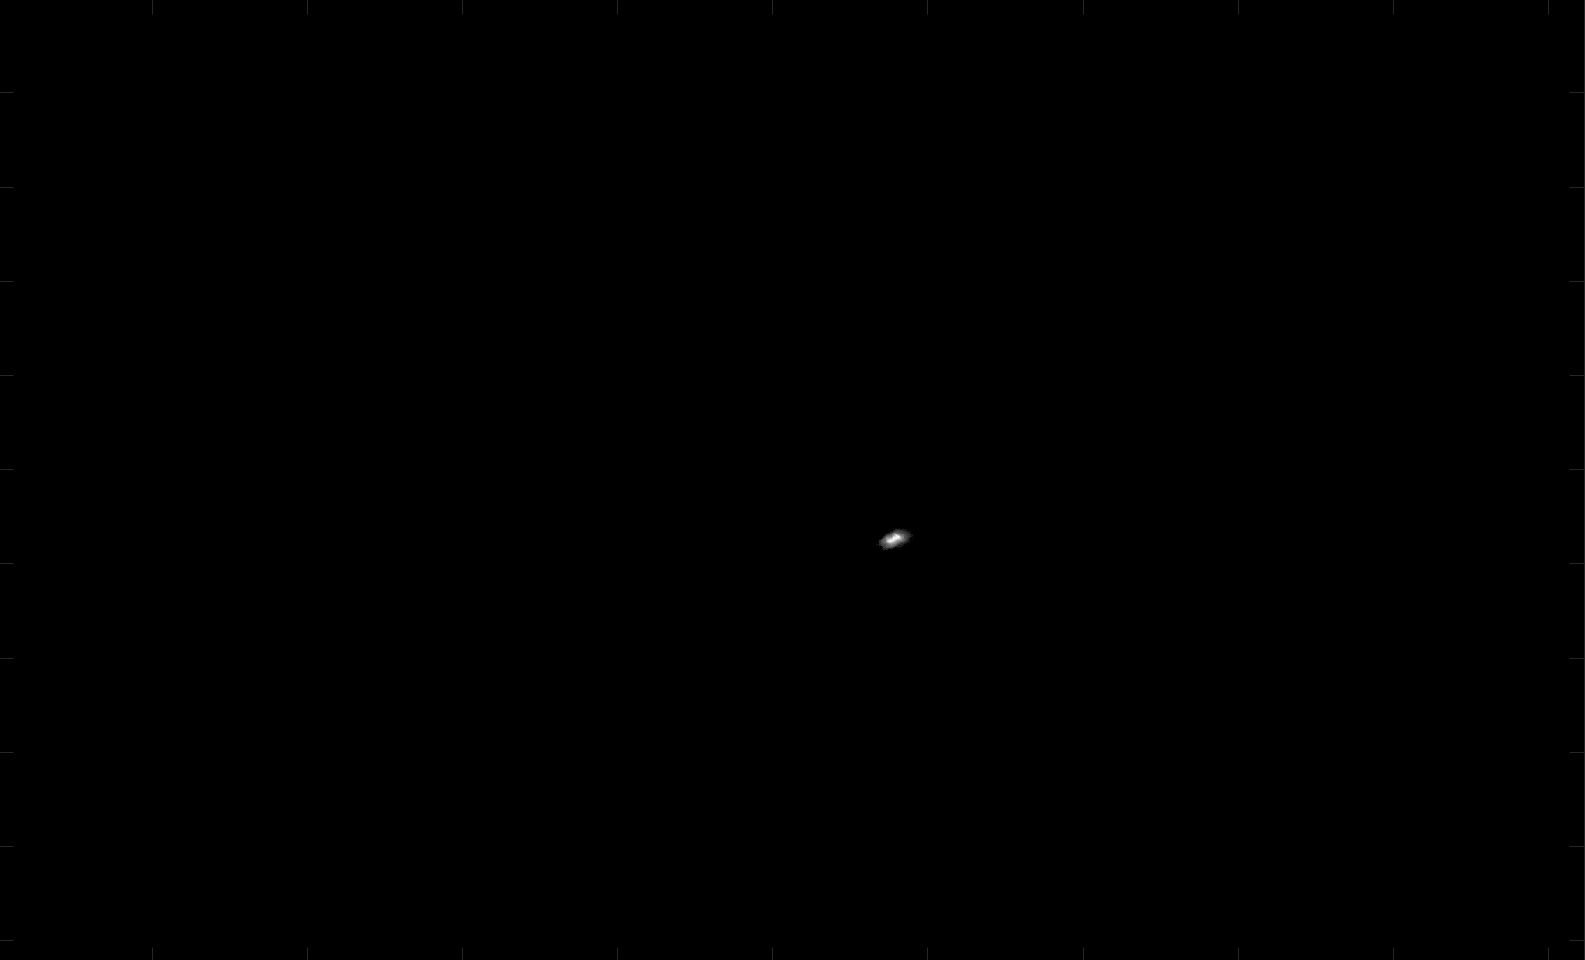
\includegraphics[width=0.45\textwidth]{med_rot_psf_12.png}
\vspace{-1em}
\caption{The sum and median images for ROXs 12, rotated so north is up and subtracting the most similar PSF.}
\end{figure}
\vspace{-1.2em}
\begin{figure}[H]
\centering
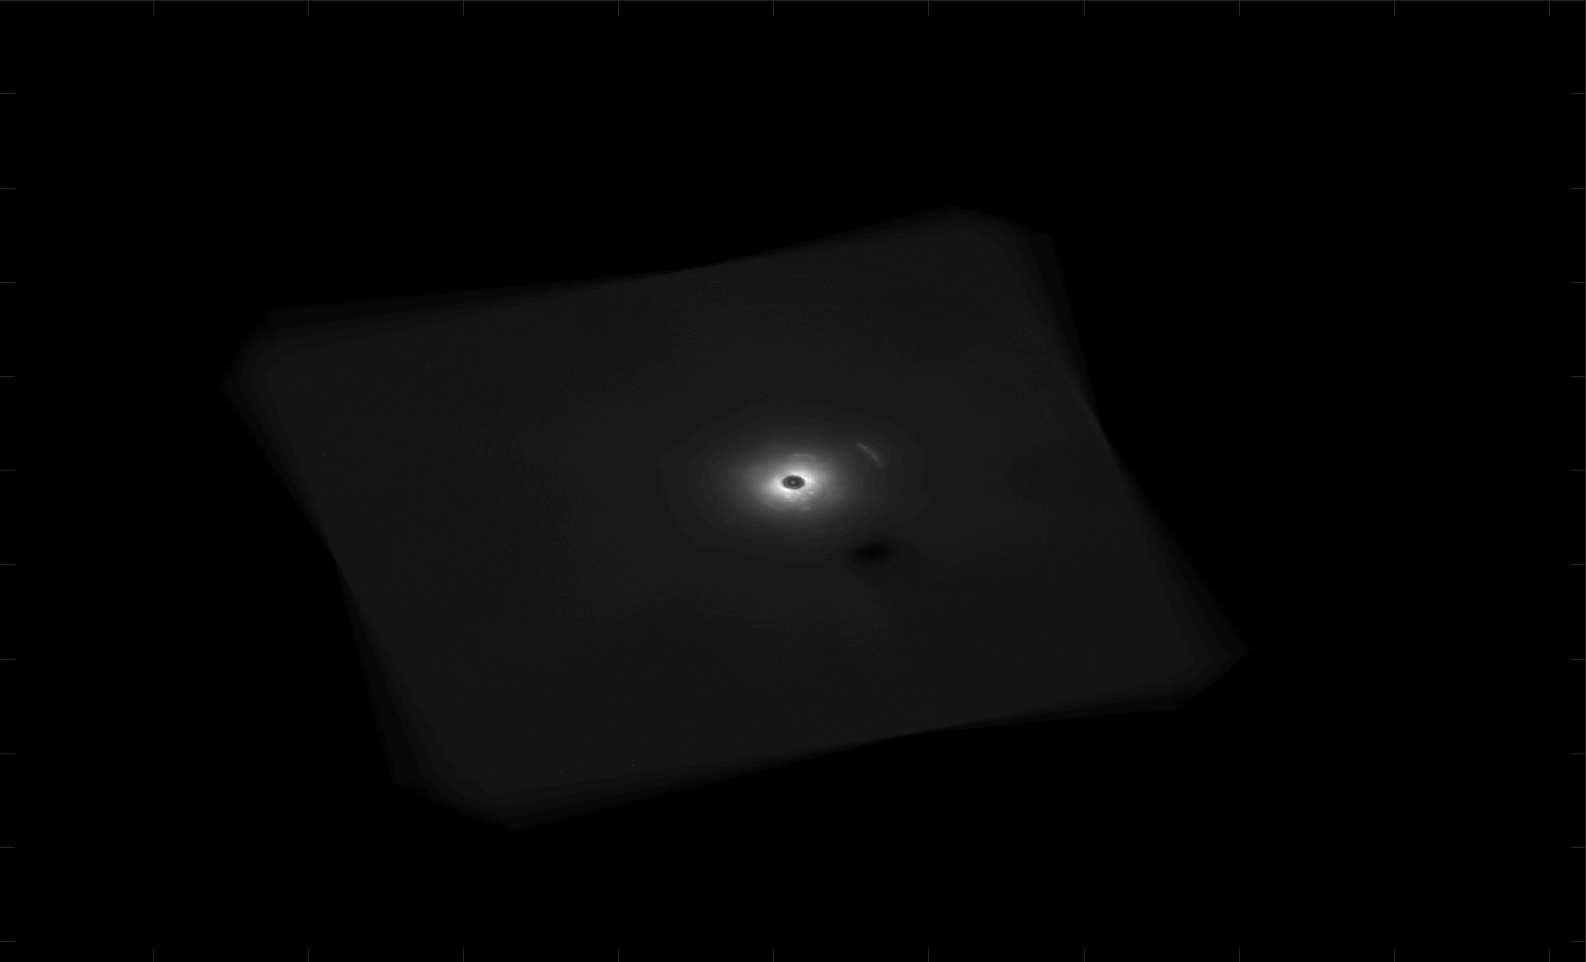
\includegraphics[width=0.45\textwidth]{sum_rot_psf_42b.png}
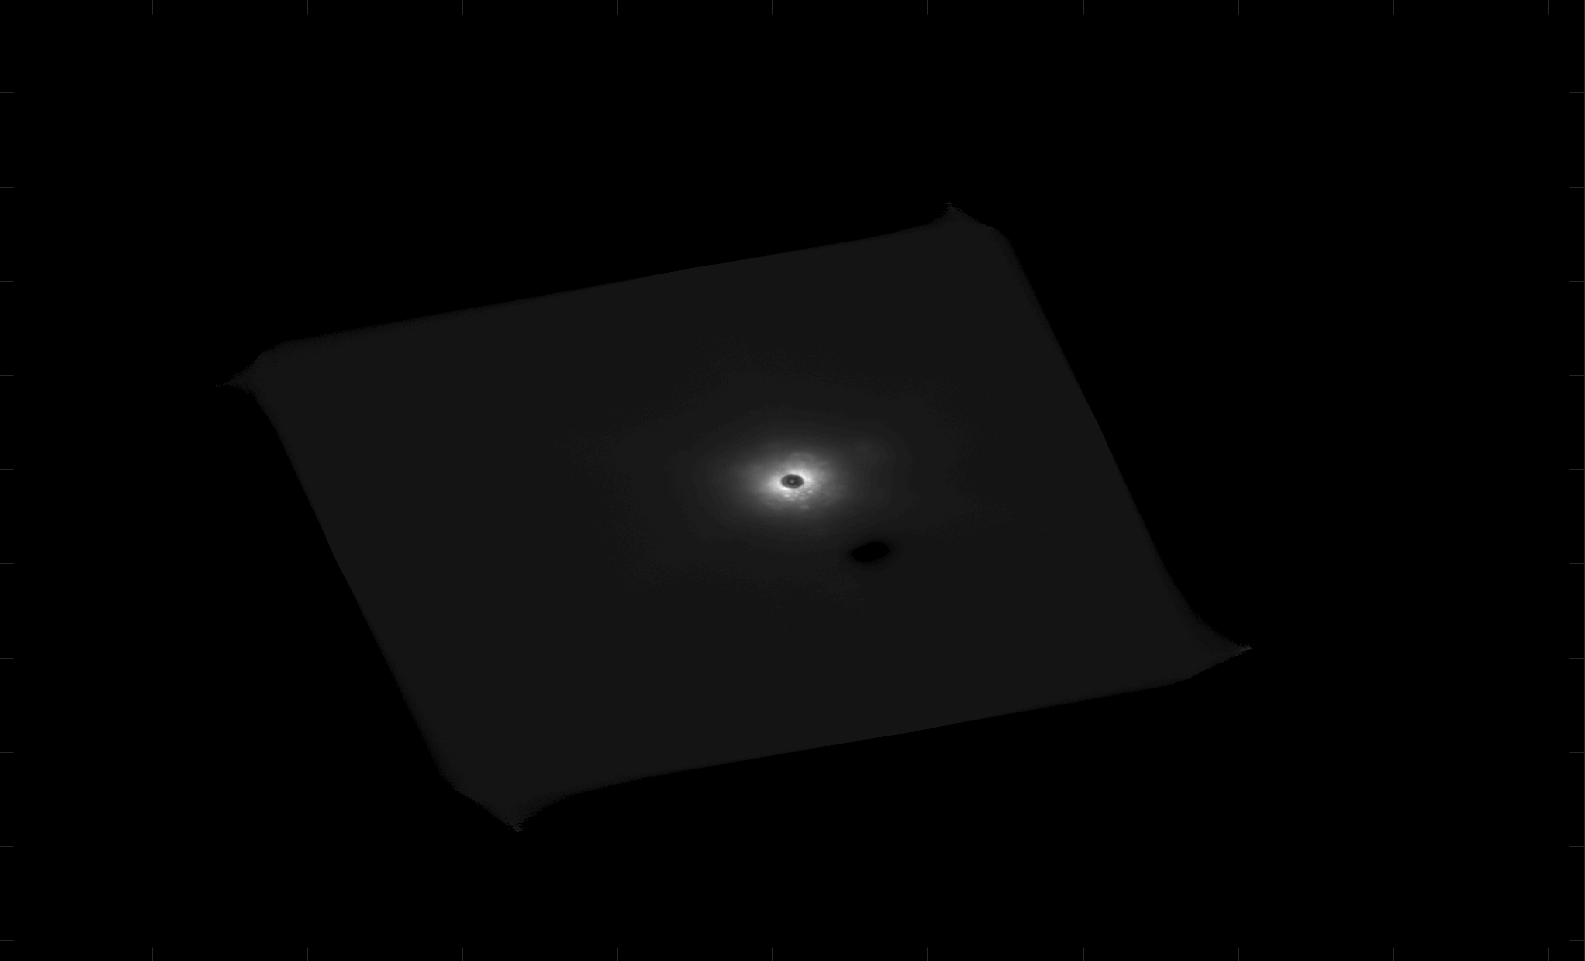
\includegraphics[width=0.45\textwidth]{med_rot_psf_42b.png}
\vspace{-1em}
\caption{The sum and median images for ROXs 42B, rotated so north is up and subtracting the most simliar PSF.}
\end{figure}


\end{document}